\documentclass[12pt]{amsart}
%\usepackage[intlimits]{amsmath}
\usepackage{setspace}
\usepackage{graphicx}
\usepackage{hyperref}
\usepackage{cite}
\usepackage{subfigure}
\usepackage{listings}
\usepackage{color}
%\usepackage[nomarkers,figuresonly]{endfloat}
\usepackage{geometry} % see geometry.pdf on how to lay out the page. There's lots.
\usepackage{paralist}
\usepackage{lscape}
\usepackage{caption}
\usepackage{lineno}
%\linenumbers

\usepackage{pgf}
\usepackage{tikz}
\usepackage{pgfplots}
%\usepackage{harvard}
\usetikzlibrary{shapes,arrows,chains,automata,fit}
\usetikzlibrary{positioning}
\usetikzlibrary{shapes.geometric,intersections}

\author{Youngung Jeong}
\address{Center for Automotive Lightweighting\\
  Materials Science and Engineering Division\\
  Materials Measurement Laboratory\\
  National Institute of Standards and Technology
}
\email[Y. Jeong]{youngung.jeong@nist.gov}

%\usepackage{authblk}
\geometry{a4paper} % or letter or a5paper or ... etc
% \geometry{landscape} % rotated page geometry
\hypersetup{
  colorlinks,%
  citecolor=blue,%,black
  filecolor=blue,%
  linkcolor=blue,%
  urlcolor=blue
}

\doublespacing

%% Custom colors
\definecolor{dkgreen}{rgb}{0,0.6,0}
%\definecolor{lime}(0,255,0)
\definecolor{gray}{rgb}{0.5,0.5,0.5}
\definecolor{mauve}{rgb}{0.58,0,0.82}
\definecolor{lightgray}{rgb}{0.83, 0.83, 0.83}
\definecolor{lightergray}{rgb}{0.90, 0.90, 0.90}
\definecolor{verylightgray}{rgb}{0.95, 0.95, 0.95}

%% not working
% \colorlet{lcfree}{Green3}
% \colorlet{lcnorm}{Blue3}
% \colorlet{lccong}{Red3}

% -------------------------------------------------
% Set up a new layer for the debugging marks, and make sure it is on
% top
\pgfdeclarelayer{marx}
\pgfsetlayers{main,marx}


%% custom lst styles
\lstdefinestyle{numbers} {numbers=left, stepnumber=1, numberstyle=\tiny, numbersep=10pt}
\lstdefinestyle{MyFrame}{backgroundcolor=\color{yellow},frame=shadowbox}

\lstdefinestyle{Fortran} {
  language=Fortran,
  aboveskip=3mm,
  belowskip=3mm,
  showstringspaces=true,
  columns=flexible,
  basicstyle={\small\ttfamily},
  numbers=left,
  numberstyle=\tiny\color{red},
  keywordstyle=\color{blue},
  commentstyle=\color{dkgreen},
  stringstyle=\color{mauve},
  breaklines=true,
  breakatwhitespace=true,
  frame=shadowbox,
  backgroundcolor=\color{verylightgray},
  tabsize=3
  }

\lstdefinestyle{sh} {
  language=bash,
  aboveskip=3mm,
  belowskip=3mm,
  showstringspaces=true,
  columns=flexible,
  basicstyle={\tiny\ttfamily},
  numbers=left,
  numberstyle=\tiny\color{blue},
  keywordstyle=\color{blue},
  commentstyle=\color{dkgreen},
  stringstyle=\color{mauve},
  breaklines=true,
  breakatwhitespace=true,
  frame=shadowbox,
  backgroundcolor=\color{lightergray},
  tabsize=3
  }

\lstdefinestyle{Python} {
  language=Python,
  aboveskip=3mm,
  frame=shadowbox,
  belowskip=3mm,
  showstringspaces=true,
  columns=flexible,
  basicstyle={\small\ttfamily},
  numbers=left,
  numberstyle=\tiny\color{red},
  keywordstyle=\color{blue},
  commentstyle=\color{dkgreen},
  stringstyle=\color{mauve},
  breaklines=true,
  breakatwhitespace=true,
  frame=shadowbox,
  backgroundcolor=\color{lightgray},
  tabsize=3}

\lstdefinestyle{inp} {
  language=bash,
  aboveskip=3mm,
  frame=shadowbox,
  belowskip=3mm,
  showstringspaces=true,
  columns=flexible,
  basicstyle={\tiny\ttfamily\scriptsize},
  numbers=left,
  numberstyle=\tiny\color{red},
  keywordstyle=\color{black},
  commentstyle=\color{dkgreen},
  stringstyle=\color{mauve},
  breaklines=true,
  breakatwhitespace=true,
  frame=shadowbox,
  backgroundcolor=\color{lightgray},
  tabsize=3
  }

\lstdefinestyle{txt} {
  aboveskip=3mm,
  frame=shadowbox,
  belowskip=3mm,
  showstringspaces=true,
  columns=flexible,
  basicstyle={\small\ttfamily},
  numbers=none,
  numberstyle=\tiny\color{red},
  keywordstyle=\color{black},
  commentstyle=\color{black},
  stringstyle=\color{black},
  breaklines=true,
  breakatwhitespace=true,
  frame=shadowbox,
  backgroundcolor=\color{lightgray},
  tabsize=3
  }

\DeclareCaptionFormat{listing}{\rule{\dimexpr\textwidth+17pt\relax}{0.4pt}\par\vskip1pt#1#2#3}
\captionsetup[lstlisting]{format=listing,singlelinecheck=false, margin=0pt, font={sf},labelsep=space,labelfont=bf}

\renewcommand\lstlistingname{Code}
% \lstset{language=Fortran,frame=none}
% \lstset{language=bash,frame=none}
% \lstset{language=Python,frame=none}

%% tikz customization
\tikzset{state/.style={rectangle,rounded corners,draw=black, very thick,
    minimum height=2em,inner sep=2pt,text centered}}
\tikzset{decision/.style={diamond,aspect=2,draw=black,very thick,
    minimum height=2em,inner sep=2pt,text centered}}
\tikzset{process/.style={circle,draw=black,very thick,
    minimum height=2em,inner sep=2pt,text centered}}
\tikzset{dot/.style={circle,draw=black,thick,
    inner sep=0pt,minimum size=4pt}}

\title{Manual for VPSC-FLD (Version 2.1.3)}
%\date{} % delete this line to display the current date

%%% BEGIN DOCUMENT

\begin{document}
\pagenumbering{arabic}

\newpage
\maketitle
\newpage
\setcounter{tocdepth}{1}
\tableofcontents
\newpage
\lstlistoflistings
\newpage
\section{Introduction}
This document is a manual for the VPSC-FLD (version 1.0), which is a numerical computer code developed in order to predict forming limit diagrams (FLD).
VPSC refers to the visco-plastic self-consistent model developed by Ricardo Lebensohn and Carlos Tom\'{e} in Los Alamos National Lab.
The VPSC-FLD program bases on a particular version of the VPSC program (version 7b).
\newline
The VPSC-FLD program comes with several Python scripts, which enable \emph{parallel} calculations for FLD simulations on the basis of Marciniak-Kuczy{\`n}ski (MK) model.
That way, the computational time for FLD calculation can be significantly reduced - this will be discussed in Section \ref{sec:paral_mode}.
Several examples are included in this manual to help users quickly learn how to execute the VPSC-FLD, assuming that the users have some experiences with the VPSC program.
For this reason, those readers with little experience on VPSC program should first read the manual of the VPSC program \cite{Tome2009} prior to using the VPSC-FLD.
If the user is already experienced with the VPSC program and only wishes to start learning the MK model, Section \ref{sec:fld} will be a good starting point.
On the other hand, those who are familiar with the MK model and want to start practicing the VPSC-FLD, reading from Sections \ref{sec:ex_single_run} through \ref{sec:sens} will be helpful.
Meanwhile, advanced users, who wish to modify/improve/contribute to the project, should refer to Section \ref{sec:subroutines}, in which an extended amount of details for some selected subroutines are given.
Also, the full package of the VPSC-FLD is available through GitHub repository. Look at Section \ref{sec:repo} for more details.
\newpage
\section{Theoretical backgrounds}
\label{sec:theory}
\subsection{Forming limit diagram}
\label{sec:fld}
In order to obtain a single FLD, the maximum deformable strains (plotted in the principal strain space consisting of two major components,
i.e., $\bar{E}_1$ and $\bar{E}_2$) are collected along various monotonic loading paths until the material's eventual failure - either necking/fracture.
By repeating the monotonic stretching along various paths, one can obtain a limit curve that delineates the safe and unsafe regions in the strain space consisting of major and minor principal strain components.
Forming limit diagram is one of the most important type of information pertaining to a sheet metal in order to measure its mechanical performance during forming processes such as stamping.
Nowadays, it is quite customary to incorporate a forming limit diagram into finite element analysis of sheet metal forming.
\newline
In order to experimentally determine the forming limits of a particular metal sheet, a large volume of material is consumed.
Therefore, an accurate model will be very useful.
To that end, there are various types of models developed over the decades.

\subsection{Marciniak Kuczy{\'n}ski approach}
\label{sec:mk}
%% variables
\newcommand*{\Cpsi}{35}%
\newcommand*{\Ctheta}{65}%
\newcommand*{\Cw}{7}%
\newcommand*{\Ch}{7}%
\newcommand*{\CtA}{0.180}%
\newcommand*{\CtB}{0.150}%
\newcommand*{\Cbw}{0.15}%
\newcommand*{\Cdisp}{\Ch/2.}%

\begin{figure}
  \includegraphics[width=0.8\textwidth]{mk_drawing3.pdf}
  \caption{Schematic views of the Marciniak-Kuczy\'{n}ski approach}
  \label{fig:mk}
\end{figure}
Back in 1960s Marciniak and Kuczy{\'n}ski developed a model to predict the forming limits when both principal stretching strains are positive \cite{Marciniak1967609}.
Since then, their model has been widely spread both in academia and industry.
The current VPSC-FLD model also follows the MK approach in order to predict the limit strains.
In what follows, a detailed illustration of the MK-approach, as implemented in the VPSC-FLD (version 1.0.1), is presented.
\newline
In the MK approach, the sheet is comprised of two regions (see Figure \ref{fig:mk}):
\begin{inparaenum}[\itshape i\upshape)]
\item homogeneous area (region \textbf{A});
\item pre-existing groove (region \textbf{B}).
\end{inparaenum}
Two parameters are introduced to characterize the geometric features of the pre-existing groove, i.e.,
\begin{inparaenum}[\itshape i\upshape)]
\item inhomogeneity parameter $f_0$ that is defined as the thickness ratio between the two regions, and
\item the angle between the pre-existing groove and the sheet's rolling direction (RD) $\psi_0$.
\end{inparaenum}
Due to this initial geometric inhomogeneity, the two regions may undergo distinct plastic history.
The region \textbf{B} may experience a faster thinning than region \textbf{A} as a result of in-plane stretching.


Note that, as shown in Figure \ref{fig:mk}, it is allowed for the stretching axes (Axes 1 and 2) to incline with respect to the orthotropic axes (RD-TD).
The inclination of the stretching axes from the orthotropic axes is quantified by $\theta$.
Likewise, the groove may incline inasmuch as $\psi$ from the stretching axes.
It should be mentioned that, in the following formalism, the reference coordinate to which tensors are referred to is the Axes 1 and 2.



A set of various monotonic loading paths, to which the homogeneous region of the sheet is subjected, can be expressed by the ratio between the major and the minor strain rate components ($\rho$).
This parameter $\rho$ alone can characterize the velocity gradients ($\bar{L}^0_{ij}$) under an arbitrary in-plane loading condition:
\begin{eqnarray}
  \label{eq:lij0}
  \bar{L}^0_{ij} =
  \begin{bmatrix}
    1 & 0 & 0 \\
    0 & \rho & 0 \\
    0 & 0 & -1-\rho
  \end{bmatrix} \mathbf{e}^\mathrm{lab}_i \otimes \mathbf{e}^\mathrm{lab}_j
\end{eqnarray}
Note that materials described by the VPSC framework behave in the domain of viscoplastic region.
Due to the plastic incompressibility only two of the diagonal components in $\bar{L}^0$ are independent.
\newline
In order to impose a constant strain rate regardless of the $\rho$ value, the above velocity gradient should be normalized:
\begin{eqnarray}
  \label{eq:lij}
  \bar{L}^\mathrm{(A)}_{ij} = \frac{\bar{L}^0_{ij}}{\dot{\bar{E}}_0^\mathrm{VM}} \dot{c},
\end{eqnarray}
in which $\dot{\bar{E}}_0^\mathrm{VM}$ is the Von Mises equivalent strain rate derived from $\bar{L}^0_{ij}$ in Eq. \ref{eq:lij0};
and $\dot{c}$ controls the strain rate.
In case of quasi-static loading conditions, $\dot{c}$ should be reasonably small.
\newline
Between the groove and the homogeneous region, an element of strain compatibility is required.
In VPSC-FLD, the formalism suggested by Hutchinson \cite{hutchinson1978sheetII,hutchinson1978sheet} is used.
Th velocity gradient pertaining to region \textbf{B} (i.e., $\bar{L}_{ij}^\mathrm{(B)}$) is adequately related to that of region \textbf{A} through
\begin{eqnarray}
  \label{eq:lij_b}
  \bar{L}^\mathrm{(B)}_{ij} = \bar{L}^\mathrm{(A)}_{ij} + v_i n_j \text{ with } i,j=1,2.
\end{eqnarray}
Note that $\bf{n}$ (in Eq. \ref{eq:lij_b}) and $\bf{t}$ (appears in below Eq. \ref{eq:forceeq}) denote the direction vectors that are normal and transverse to the groove, respectively, as shown in Figure \ref{fig:mk}.
Therefore $\bf{n}$ and $\bf{t}$ are $[\cos(\psi-\theta), \sin(\psi-\theta),0] $ and $[-\sin(\psi-\theta), \cos(\psi-\theta), 0]$, respectively.
\newline
The velocity components ($v_i$) are initially unknown for a given incremental step, thus should be numerically determined based on the force equilibrium condition across the boundary between the two regions.
\begin{subequations}
  \label{eq:forceeq}
  \begin{eqnarray}
    |f\  \mathbf{n} \cdot \bar{\mathbf{\Sigma}}^\mathrm{(B)} \cdot \bf{n} - \bf{n} \cdot \bar{\mathbf{\Sigma}}^\mathrm{(A)} \cdot \bf{n} | < Err_1 \\
    |f\  \mathbf{n} \cdot \bar{\mathbf{\Sigma}}^\mathrm{(B)} \cdot \bf{t} - \bf{n} \cdot \bar{\mathbf{\Sigma}}^\mathrm{(A)} \cdot \bf{t} | < Err_2
  \end{eqnarray}
\end{subequations}
in which $\bar{\mathbf{\Sigma}}^\mathrm{(A)}$ and $\bar{\mathbf{\Sigma}}^\mathrm{(B)}$ are the flow stresses of the regions \textbf{A} and \textbf{B}, respectively.
The numerical tolerances (i.e., $\mathrm{Err_1}$ and $\mathrm{Err_2}$) should be sufficiently smaller than the values of $\bar{\mathbf{\Sigma}}^\mathrm{(A)}$ and $\bar{\mathbf{\Sigma}}^\mathrm{(B)}$.
\newline
This procedure is repeated until the onset of forming limit.
The criterion for the onset of forming limit is determined by thinning rate differential between the two regions.
In VPSC-FLD, the onset of the forming limit is defined as:
\begin{eqnarray}
  \label{eq:crt}
  \frac{\dot{\bar{E}}_{33}^\mathrm{(B)}}{\dot{\bar{E}}_{33}^\mathrm{(A)}}>C.
\end{eqnarray}
Justification of this criterion is not pursued here, which is beyond the scope of the current document.



\subsection{Implementation of MK into the VPSC framework}
\label{sec:imple}
In current Section, discussions on the MK model continue with focus on the interface with the VPSC framework.
Focus of current Section is primarily regarding the condition of force equilibrium, which was discussed earlier in Section \ref{sec:fld}.
Detailed discussion of the computational procedure will be given in a latter part of this manual - see Section \ref{sec:intf}.
Only a brief discussion is made in what follows.
\newline
In the VPSC-FLD program, in order to find the forming limits, two separate simulations are required for regions \textbf{A} and \textbf{B}, respectively.
In order to obtain the necessary information to solve the force equilibrium in Eq. \ref{eq:forceeq},
the constitutive flow responses of region \textbf{A} are recorded at each and every incremental step (N) until a sufficiently large deformation is reached.
Then, simulations for region \textbf{B} start with reading the constitutive responses of the region \textbf{A}, which is restored from a binary file created by the previous simulation.
The binary file should include constitutive properties of region \textbf{A},i.e., $\bar{E}^\mathrm{(A)}$, $\bar{\Sigma}^\mathrm{(A)}$, and $\bar{L}^\mathrm{(A)}$.
\newline
This is useful, as simulation of \textbf{B} often require a lot more number of simulations that the case of region \textbf{A}.
For example, simulations for region \textbf{B} may require probings based on various sets of $f_0$ and $\psi_0$.
Meanwhile, flow behavior of region \textbf{A} is independent of these values, thus saving flow behavior of the region \textbf{A} one time and reusing it repeatedly may be advantageous.
The drawback is that some additional computational time is required in order to obtain the constitutive responses of region \textbf{A} until a sufficiently large plastic deformation.
However, usually computation time required for region \textbf{A} is significantly lower than that for region \textbf{B}.
\newline
Nevertheless, given the material states of the region \textbf{A},
proper flow stress response pertaining to region \textbf{B} ($\bar{\mathbf{\Sigma}}^\mathrm{(B)}$) is \emph{numerically} determined while satisfying Eq. \ref{eq:forceeq}.
To do so, the above two force equilibrium conditions in Eq. \ref{eq:forceeq} are rearranged to provide the two objective functions $F_{i}$ with $i=1, 2$:
\begin{subequations}
  \label{eq:objf}
  \begin{eqnarray}
    F_1 = f \mathbf{n} \cdot \bar{\mathbf{\Sigma}}^\mathrm{(B)} \cdot \bf{n} - \bf{n} \cdot \bar{\mathbf{\Sigma}}^\mathrm{(A)} \cdot \bf{n} \\
    F_2 = f \mathbf{n} \cdot \bar{\mathbf{\Sigma}}^\mathrm{(B)} \cdot \bf{t} - \bf{n} \cdot \bar{\mathbf{\Sigma}}^\mathrm{(A)} \cdot \bf{t}.
  \end{eqnarray}
\end{subequations}
\newline
Both $F_1$ and $F_2$ should be minimized to meet the force equilibrium condition for each and every incremental step.
Note $F_1$ and $F_2$ are dependent on $v_1$ and $v_2$ through the formalism in Eq. \ref{eq:lij_b}.
To that end, a $2\times2$ Jacobian matrix $J_{ij}$ is required to numerically minimize $F_i$ to find proper $v_j$.
Minimization of $F_i$ is conducted based on the Newton-Raphson scheme, provided that the Jacobian matrix $J_{ij}$ is available.
Unfortunately, the analytic solution of the Jacobian matrix is not known.
Therefore, a numerically estimated Jacobian is used in the VPSC-FLD, which is defined as follows:
\begin{subequations}
  \label{eq:jac}
  \begin{eqnarray}
    J_{11}^{(k)} = \frac{F_1(v_1+\delta{v},v_2          ) - F_1(v_1,v_2)}{\delta{v}} \\
    J_{12}^{(k)} = \frac{F_1(v_1          ,v_2+\delta{v}) - F_1(v_1,v_2)}{\delta{v}} \\
    J_{21}^{(k)} = \frac{F_2(v_1+\delta{v},v_2          ) - F_2(v_1,v_2)}{\delta{v}} \\
    J_{22}^{(k)} = \frac{F_2(v_1          ,v_2+\delta{v}) - F_2(v_1,v_2)}{\delta{v}}
  \end{eqnarray}
\end{subequations}
in which variation of the objective function is induced by altering the velocity gradient $v_i$ in the amount of $\delta{v}$.
In order to accurately represent the locality of the Jacobian matrix for the given $v_i$, $\delta{v}$ should be sufficiently small.
However, an exceedingly low value for $\delta{v}$ may lead to numerical divergence according to the current author's experience.
\newline
Once the Jacobian matrix is identified, one can iteratively updates $v_i$ according to the conventional Newton-Raphson method.
\begin{eqnarray}
  \label{eq:vi_update}
  v_i^{(k+1)} = v_i^{(k)} - [J^{(k)}]^{-1}_{ij}F^{(k)}_j,
\end{eqnarray}
with $k$ indicating the $k$-th iterative step.
The iterative estimation for $v_i$ is carried out until the force equilibrium condition is satisfied.
A schematic depiction of the above numerical scheme is shown in Fig. \ref{fig:nr}, which illustrates how $v_i$ for the next iterative step ($k+1$) is obtained and so forth.
\begin{figure}
  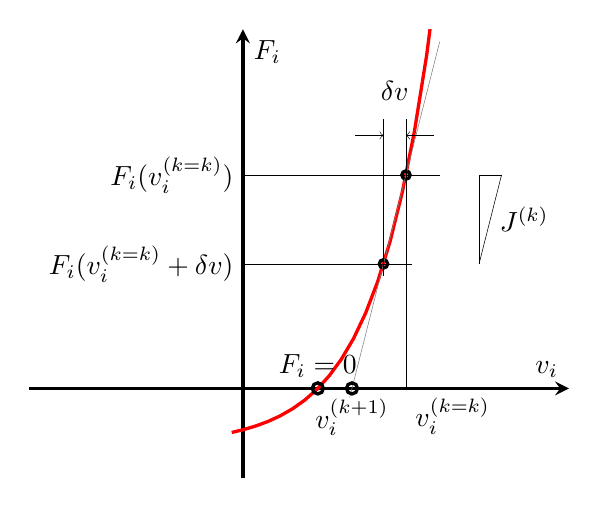
\begin{tikzpicture}[]
    \begin{axis}[axis equal,
      xmin=-3.0,ymin=-0.2,
      xmax=5,ymax=5,axis lines=middle,
      very thick,
      enlargelimits,
      xtick=\empty,
      ytick=\empty,
      xlabel={$v_i$},
      ylabel={$F_i$},
      ]
      \addplot[red, very thick,domain=-0.2:5]{pow(2.7182,x+2)/28.-1};

      %% true solution
      \draw (axis cs:1.332,0) circle [radius=2.0pt, fill=blue] node[above] {$F_i=0$};
      %% two points where slope is estimated
      \draw (axis cs:2.9,3.7960) circle [radius=1.5pt];
      \draw (axis cs:2.5,2.2150) circle [radius=1.5pt];
      %% anchor for F^(k)
      \draw[-,very thin]  (axis cs:3.5,3.796) -- (axis cs:0,3.796) node[left,black] {$F_i(v_i^{(k=k)})$};
      %% anchor for F^(k+1)
      \draw[-,very thin]  (axis cs:3.0,2.2150) -- (axis cs:0,2.2150) node[left,black] {$F_i(v_i^{(k=k)}+\delta{v})$};
      %% Extrapolated Slope
      \draw[-,very thin, gray] (axis cs:1.9,-0.157) -- (axis cs:3.5,6.168);
      %% anchor for v^(k+1)
      \draw (axis cs:1.9397,0) circle [radius=2.0pt] node[below] {$v_i^{(k+1)}$};
      %% anchor for v^(k)
      \draw[-,very thin] (axis cs:2.9,3.796) -- (axis cs:2.9,0.) node[below right] {$v_i^{(k=k)}$};
      %% Gap for delta v
      \draw[-,very thin] (axis cs:2.9, 2.0) -- (axis cs:2.9, 4.8);
      \draw[-,very thin] (axis cs:2.5, 2.0) -- (axis cs:2.5, 4.8);
      \draw[->,very thin] (axis cs:2.0, 4.5) -- (axis cs:2.5,4.5);
      \draw[<-,very thin] (axis cs:2.9, 4.5) -- (axis cs:3.4,4.5);
      \node at (axis cs:2.7, 5.3) {$\delta{v}$};
      %% Jacobian triangle
      \draw[-,very thin] (axis cs:4.2,2.2150) to node[right,black]{$J^{(k)}$} (axis cs:4.6,3.796);
      \draw[-,very thin] (axis cs:4.2,2.2150) -- (axis cs:4.2,3.796) -- (axis cs:4.6,3.796);
    \end{axis}
  \end{tikzpicture}
  \caption{Schematic view on the Newton Raphson numerical procedure using the forward Jacobian - the objective function of current interests is actually in the form of a surface, which is mapped in the space of $v(v_1,v_2)$}
  \label{fig:nr}
\end{figure}
Users can easily customize the numerical parameters related with the above procedure such as $\delta{v}, e_1$ and $e_2$ in file \verb$FLD_nu.in$.
However, care should be taken as the numerical stability may rely on those parameters.
\newline
Due to plastic deformation, the geometry of the sheet may alter as illustrated in Figure \ref{fig:mk2}.
Following \cite{kuroda2000forming}, below rule is used to update the orientation of the band.

\begin{eqnarray}
  \label{eq:fpsi_update1}
  \boldsymbol{n}=\frac{1}{\sqrt{t_1^2+t_2^2}}
  \begin{pmatrix}
    t_2\\
    t_1
  \end{pmatrix}
\end{eqnarray}
where the tangential vector $\boldsymbol{t}$ is updated according to the deformation gradient tensor $\boldsymbol{F}$:
\begin{eqnarray}
  \label{eq:fpsi_update2}
t_i = F_{ij} t^0_j.
\end{eqnarray}
Note that $t^0$ is the initial tangential vector as depicted in Figure \ref{fig:mk}.
Thus the current angle of the band ($\psi$) is determined as:
\begin{eqnarray}
  \label{eq:fpsi_update3}
  \psi = \text{atan2}(n_2,n_1),
\end{eqnarray}
where atan2 is a standard function in FORTRAN to calculates the appropriate quadrant angle for coordinates (y,x).


% The update rule for $\psi$ is valid only when $\theta=0^\circ{}$ or $90^\circ{}$.
\newpage
\begin{figure}%[width=\textwidth,hbtp]
  %% variables
  \renewcommand*{\Cpsi}{35}%
  \renewcommand*{\Ctheta}{0}%
  \renewcommand*{\Cw}{5.00}%
  \renewcommand*{\Ch}{5.00}%
  \renewcommand*{\CtA}{0.180}%
  \renewcommand*{\CtB}{0.150}%
  \renewcommand*{\Cbw}{0.15}%
  \renewcommand*{\Cdisp}{\Ch/4.}%

  \begin{subfigure}[]{}
    \begin{tikzpicture}[>=stealth]
      %% Top view
      %% sheet
      \draw [ultra thick] (-\Cw/2., -\Ch/2.) rectangle (\Cw/2, \Ch/2.){};
      %% inclined Band
      %% band function y = -1/tan(\Cpsi) {x)
      %% x = -(y)* tan(\Cpsi)
      \path[fill=gray, draw=black, very thin] ({-\Ch/2.*tan(\Cpsi) - \Cbw * cos(\Cpsi)},\Ch/2.) -- ({\Ch/2. * tan(\Cpsi) - \Cbw*cos(\Cpsi)},-\Ch/2.)-- ({\Ch/2. * tan(\Cpsi) + \Cbw*cos(\Cpsi)},-\Ch/2.) -- ({-\Ch/2.*tan(\Cpsi) + \Cbw * cos(\Cpsi)},\Ch/2.)  -- ({-\Ch/2.*tan(\Cpsi) - \Cbw * cos(\Cpsi)},\Ch/2.)  {};

      %% RD-TD axes
      \draw[<->, red] (0,\Ch/4.) node[above]{$\mathbf{e}_2\parallel$TD}-- (0,0) -- (\Ch/4.,0) node[below right]{$\mathbf{e}_1\parallel$RD};
      %% n-t axes
      \draw[<->, blue] ({cos(\Cpsi)*\Ch/4.}, {sin(\Cpsi)*\Ch/4.}) node[above]{$\mathbf{n}_0$} -- (0,0) -- ({-sin(\Cpsi)*\Ch/4.}, {cos(\Cpsi)*\Ch/4.}) node[left]{$\mathbf{t}_0$} {};
      % %% Stretching axes
      % \draw[<->, magenta] (-\Ch/4.,0) node[left]{2} -- (-\Ch/4.,-\Ch/4.)  -- (0,-\Ch/4.) node[below right]{1};
      %% psi arc
      \draw[->, black] (0.5,0) node [above right] {$\psi_0$} arc (0:\Cpsi:0.5);
      \draw[->, black] (0,0.5) node [above left]  {$\psi_0$} arc (90:90+\Cpsi:0.5);
      %% Cross-sectional view (B)
      \draw[-, gray, thin, fill] (-\CtA,  -\Ch/2. - \Cdisp - \CtA/2+\CtB/2) rectangle (+\CtA,  -\Ch/2. - \Cdisp - \CtA/2-\CtB/2) {};
      %% Cross-sectional view (A)
      \draw[-, black,ultra thick, fill=white] (-\Cw/2., -\Ch/2. -\Cdisp) rectangle (0-\CtA,-\Ch/2. -\Cdisp -\CtA){};
      \draw[-, black,ultra thick, fill=white] ( \Cw/2., -\Ch/2. -\Cdisp) rectangle (0+\CtA,-\Ch/2. -\Cdisp -\CtA){};

      %% Thickness A Arrow
      \draw[->,black]  (-\Cw/4.,-\Ch/2.-\Cdisp + 0.2) -- (-\Cw/4.,-\Ch/2.-\Cdisp);
      \draw[<-,black] (-\Cw/4.,-\Ch/2.-\Cdisp-\CtA) -- (-\Cw/4., -\Ch/2.-\Cdisp-\CtA-0.2) ;
      %% Thickness B Arrow
      \draw[->,black] (0,-\Ch/2.-\Cdisp-\CtA/2.+\CtB/2.+0.2) -- (0,-\Ch/2.-\Cdisp-\CtA/2.+\CtB/2.);
      \draw[<-,black] (0,-\Ch/2.-\Cdisp-\CtA/2.-\CtB/2.)     -- (0,-\Ch/2.-\Cdisp-\CtA/2.-\CtB/2.-0.2);
      %% parameter f

      %% Labeling
      \node at (+\Cw/4,             \Ch/2.*0.9) {Region \textbf{A}};
      \node at (-\Cw/4,            -\Ch/2.*0.9) {Region \textbf{A}};
      \node at (-\Cw/4., -\Ch/2.-\Cdisp + 0.2)[left]{$t_0^\mathrm{(A)}$};
      \node at (0,       -\Ch/2.-\Cdisp + 0.2)[left]{$t_0^\mathrm{(B)}$};
      \node[right] at ( \Cw/2    , -\Ch/2.-\Cdisp){$f_0=t_0^\mathrm{(B)}/t_0^\mathrm{(A)}$};

    \end{tikzpicture}

    % \caption{Initial}
    % \label{fig:mk2_a}
  \end{subfigure}
  \vspace{40pt}

  \renewcommand*{\Cpsi}{49.1}%
  \renewcommand*{\Ctheta}{0}%
  \renewcommand*{\Cw}{7.50}%
  \renewcommand*{\Ch}{5.00}%
  \renewcommand*{\CtA}{0.180}%
  \renewcommand*{\CtB}{0.150}%
  \renewcommand*{\Cbw}{0.15}%
  \renewcommand*{\Cdisp}{\Ch/4.}%

  \begin{subfigure}[]{}%{0.49\textwidth}
    \begin{tikzpicture}[>=stealth]
      %% Top view
      %% sheet
      \draw [ultra thick] (-\Cw/2., -\Ch/2.) rectangle (\Cw/2, \Ch/2.){};
      %% inclined Band
      % \path[fill=gray, draw=black, very thin] (-\Cw/2., {-tan(\Cpsi)*\Cw/2.+\Cbw/cos(\Cpsi)}) -- ( \Cw/2. ,{ tan(\Cpsi)*\Cw/2.+\Cbw/cos(\Cpsi)}) -- ( \Cw/2. ,{ tan(\Cpsi)*\Cw/2.-\Cbw/cos(\Cpsi)}) node [right]{Region \textbf{B}} -- (-\Cw/2., {-tan(\Cpsi)*\Cw/2.-\Cbw/cos(\Cpsi)}) -- (-\Cw/2., {-tan(\Cpsi)*\Cw/2.+\Cbw/cos(\Cpsi)}) {};
      %% band function y = -1/tan(\Cpsi) {x)
      %% x = -(y)* tan(\Cpsi)
      \path[fill=gray, draw=black, very thin] ({-\Ch/2.*tan(\Cpsi) - \Cbw * cos(\Cpsi)},\Ch/2.) -- ({\Ch/2. * tan(\Cpsi) - \Cbw*cos(\Cpsi)},-\Ch/2.)-- ({\Ch/2. * tan(\Cpsi) + \Cbw*cos(\Cpsi)},-\Ch/2.) -- ({-\Ch/2.*tan(\Cpsi) + \Cbw * cos(\Cpsi)},\Ch/2.)  -- ({-\Ch/2.*tan(\Cpsi) - \Cbw * cos(\Cpsi)},\Ch/2.)  {};

      %% Stretching axes
      \draw[<->, red] (0,\Ch/4.) node[above]{$\mathbf{e}_2\parallel$TD}-- (0,0) -- (\Ch/4.,0) node[below right]{$\mathbf{e}_1\parallel$RD};
      %% n-t axes
      \draw[<->, blue] ({cos(\Cpsi)*\Ch/4.}, {sin(\Cpsi)*\Ch/4.}) node[above]{$\mathbf{n}$} -- (0,0) -- ({-sin(\Cpsi)*\Ch/4.}, {cos(\Cpsi)*\Ch/4.}) node[left]{$\mathbf{t}$} {};
      %% psi arc
      \draw[->, black] (0.5,0) node [above right] {$\psi$} arc (0:\Cpsi:0.5);
      \draw[->, black] (0,0.5) node [above left]  {$\psi$} arc (90:90+\Cpsi:0.5);
      %% Cross-sectional view (B)
      \draw[-, gray, thin, fill] (-\CtA,  -\Ch/2. - \Cdisp - \CtA/2+\CtB/2) rectangle (+\CtA,  -\Ch/2. - \Cdisp - \CtA/2-\CtB/2) {};
      %% Cross-sectional view (A)
      \draw[-, black,ultra thick, fill=white] (-\Cw/2., -\Ch/2. -\Cdisp) rectangle (0-\CtA,-\Ch/2. -\Cdisp -\CtA){};
      \draw[-, black,ultra thick, fill=white] ( \Cw/2., -\Ch/2. -\Cdisp) rectangle (0+\CtA,-\Ch/2. -\Cdisp -\CtA){};

      %% Thickness A Arrow
      \draw[->,black]  (-\Cw/4.,-\Ch/2.-\Cdisp + 0.2) -- (-\Cw/4.,-\Ch/2.-\Cdisp);
      \draw[<-,black] (-\Cw/4.,-\Ch/2.-\Cdisp-\CtA) -- (-\Cw/4., -\Ch/2.-\Cdisp-\CtA-0.2) ;
      %% Thickness B Arrow
      \draw[->,black] (0,-\Ch/2.-\Cdisp-\CtA/2.+\CtB/2.+0.2) -- (0,-\Ch/2.-\Cdisp-\CtA/2.+\CtB/2.);
      \draw[<-,black] (0,-\Ch/2.-\Cdisp-\CtA/2.-\CtB/2.)     -- (0,-\Ch/2.-\Cdisp-\CtA/2.-\CtB/2.-0.2);
      %% parameter f

      %% Labeling
      \node at (+\Cw/4,             \Ch/2.*0.9) {Region \textbf{A}};
      \node at (-\Cw/4,            -\Ch/2.*0.9) {Region \textbf{A}};
      \node at (-\Cw/4., -\Ch/2.-\Cdisp + 0.2)[left]{$t^\mathrm{(A)}$};
      \node at (0,       -\Ch/2.-\Cdisp + 0.2)[left]{$t^\mathrm{(B)}$};
      \node[right] at ( \Cw/2    , -\Ch/2.-\Cdisp){$f=t^\mathrm{(B)}/t^\mathrm{(A)}$};

    \end{tikzpicture}
  \end{subfigure}
  \caption{Changes in $\psi$ and $f$: (a) Initial; (b) After a plane-strain deformation (i.e., $\rho=0$)}
  \label{fig:mk2}
\end{figure}

\subsection{Stress rate control}
\label{sec:imple_alpha}
In the current section, the implementation of the stress ratio control is given.
The stress ratio $\alpha$ is defined as:
\begin{eqnarray}
  \alpha=\frac{\bar{\Sigma}_{1}}{\bar{\Sigma}_{2}}.
\end{eqnarray}
For the given $\alpha$, the corresponding $\rho$ is numerically determined.
To that end, the initial guess on $\rho$ is determined on the basis of Von Mises yield function with the associated flow rule:

\begin{eqnarray}
  d\bar{E}_{ij} = d\lambda \frac{\partial \Phi}{\partial \bar{\Sigma}_{ij}}
\end{eqnarray}
where the plastic potential $\Phi$ is simply replaced with the Von Mises yield function, i.e.,:
\begin{eqnarray}
  \Phi^\mathrm{VM} = (\frac{3}{2} \bar{S}_{ij})^{\frac{1}{2}}
\end{eqnarray}
where $\boldsymbol{\bar{S}}$ denotes the deviatoric stress.
Thus, under this condition, the direction of plastic strain tensor is:
\begin{subequations}
  \label{eq:asf}
  \begin{eqnarray}
    d\bar{E}_{ij} = d\lambda \sqrt{\frac{3}{2}\bar{S}_{ij}}, \\
    \bar{S}_{ij} = \frac{d\bar{E}_{ij}}{d\lambda} \sqrt{\frac{2}{3}}.
  \end{eqnarray}
\end{subequations}
Meanwhile, the Cauchy stress state can be parameterized using $\alpha$ in the case of plane-stress condition:
\begin{eqnarray}
\bar{\Sigma}_{ij} =
\begin{bmatrix}
  \bar{\Sigma}_{11} &0                       &0\\
  0                 &\alpha \bar{\Sigma}_{11}&0\\
  0                 &0                       &0
\end{bmatrix},
\end{eqnarray}
which can be expressed with the deviatoric terms through:
\begin{eqnarray}
\bar{S}_{ij} =
\begin{bmatrix}
  \bar{\Sigma}_{11} &0                       &0\\
  0                 &\alpha \bar{\Sigma}_{11}&0\\
  0                 &0                       &0
\end{bmatrix}
-\frac{\delta_{ij}}{3} (1+\alpha) \bar{\Sigma}_{11}.
\end{eqnarray}
In the matrix representation the deviatoric stress tensor is in the form of following:
\begin{eqnarray}
\bar{S}_{ij} =
\begin{bmatrix}
  (2/3-1/3\alpha)\bar{\Sigma}_{11} &0                       &0\\
  0                                &(2/3\alpha - 1/3) \bar{\Sigma}_{11}&0\\
  0                 &0                       &-1/3(1+\alpha) \bar{\Sigma}_{11}
\end{bmatrix}
\end{eqnarray}
One can define the incremental form of strain rate tensor:
\begin{eqnarray}
  d\bar{E}_{ij} = \sqrt{3/2}\  \bar{\Sigma}_{11}
\begin{bmatrix}
  (2/3-1/3\alpha) &0                       &0\\
  0                                &(2/3\alpha - 1/3)&0\\
  0                 &0                       &-1/3(1+\alpha)
\end{bmatrix}
d\lambda.
\end{eqnarray}

Assuming that there's no rigid body rotation, $\bar{L}_{ij}^0$ defined earlier in Equation \ref{eq:lij0} can be a function of
$\alpha$:
\begin{eqnarray}
  \label{eq:lij0_alpha}
  \bar{L}^0_{ij} =
  \begin{bmatrix}
  (2/3-1/3\alpha) &0                       &0\\
  0                                &(2/3\alpha - 1/3)&0\\
  0                 &0                       &-1/3(1+\alpha)
  \end{bmatrix},
\end{eqnarray}
Therefore, the initial guess on $\rho$ (i.e., $\rho^0$) for the given $\alpha$ using Von Mises yield function and the associated flow rule is:
\begin{eqnarray}
  \label{eq:rho_alpha}
\rho^0 = (2 \alpha - 1) / (2 - 1 \alpha)
\end{eqnarray}

Of course, this is merely an initial guess on $\rho$.
The appropriate value of $\rho$ should be numerically found by minimizing the appropriate objective function, which is defined below:
\begin{eqnarray}
  \label{eq:f_obj_alpha}
  f = |\bar{\Sigma}_{22} - \alpha \bar{\Sigma}_{11}|.
\end{eqnarray}
If $f$ with the initially guess $\rho^0$ following above does not give an appropriate value, Newton Raphson method is used to update the $\rho$.
The forward Jacobian can be determined by altering $\rho$ by:
\begin{eqnarray}
  \label{eq:rho_var}
  \rho^1 = \rho^0 + \delta\rho
\end{eqnarray}
with $\delta\rho$ being negligibly small.
The forward Jacobian is determined as:
\begin{eqnarray}
  \label{eq:jacob_alpha}
  J^0 = \frac{f(\rho^1) - f(\rho^0)}{\delta\rho}.
\end{eqnarray}
The guessed value for $\rho$ for the $n$-th iterative step is:
\begin{eqnarray}
  \label{eq:update_rho}
  \rho^{n+1} = \rho^n - f^n/J^n.
\end{eqnarray}

\newpage
\subsection{Direct approach; available from VPSC-FLD v2.1}
\label{sec:imple_da}
This section focuses on a numerical procedure (so called the \emph{direct approach}) discussed in \cite{schwindt201562}.
This approach makes use of the internal solver of VPSC when determining the boundary condition for the band, that is associated with the material response originated from the region A.
The boundary condition for the method used in \ref{eq:lij_b} requires an additional Newton-Raphson loop to determine the $v_i$ components to meet with the force equilibrium condition in Eq. \ref{eq:forceeq}.
In the direct approach, the numerical determination of $v_i$ is not necessary.
The basic idea is to rotate the reference axes of the band region inclined by the angle $\psi$, such that the normal ($\mathbf{n}$) and transverse ($\mathbf{t}$) directions of the band coincide with the new reference frame to which the boundary condition of region B is referenced.
That way, one of the stress components is given, and the two components of velocity gradients are provided from region A results as well.
The detailed procedure is given in \cite{schwindt201562}.
This strategy has been implemented to VPSC-FLD v2.1.

First, the boundary condition for region A is dictated in terms of velocity gradient $\mathbf{L}^{(A)}$.
\begin{eqnarray}
  \label{eq:lij0_da}
  \bar{L}^{\mathrm{(A)}}_{ij}= c
  \begin{bmatrix}
    1 & *    & 0 \\
    0 & \rho & 0 \\
    0 & 0    & -1 -\rho
  \end{bmatrix}
  e^\mathrm{lab}_i \otimes e^\mathrm{lab}_j
\end{eqnarray}
where $\bar{L}^{\mathrm{(A)}}_{12}$ is {\it relaxed} that is denoted as *.
As a result, the following resulting stress is expected:
\begin{eqnarray}
  \label{eq:sigma_da}
  \bar{\Sigma}^{\mathrm{(A)}}_{ij}=
  \begin{bmatrix}
    \bar{\Sigma}^{\mathrm{(A)}}_{11} & 0                                & 0  \\
    -                                & \bar{\Sigma}^{\mathrm{(A)}}_{22} & 0  \\
    \text{symmetry}                  & -                                & 0
  \end{bmatrix}
  e^\mathrm{lab}_i \otimes e^\mathrm{lab}_j.
\end{eqnarray}
In the above, the basis vectors (denoted as $\mathbf{e}^\mathrm{(r)}$) are attached with the stretching axes 1 and 2.
In the DA approach, the tensorial properties are referred to the Cartensian coordinates with basis vectors $\mathbf{e}^\mathrm{(nt)}$ attached to $\mathbf{n}$ and $\mathbf{t}$ directions.

When $\bar{L}^\mathrm{(A)}_{ij}$ is transformed to $\bar{L}^\mathrm{(A,grv)}_{ij}$, the velocity gradient pertaining to region B should be written as:
\begin{eqnarray}
  \label{eq:lij0_da_b}
  \bar{L}^{\mathrm{(B,grv)}}_{ij}= c
  \begin{bmatrix}
    * & \bar{L}^\mathrm{(A,grv)}_{12}  & 0 \\
    * & \bar{L}^\mathrm{(A,grv)}_{22}  & 0 \\
    * & *    & *
  \end{bmatrix}
  e^\mathrm{(nt)}_i \otimes e^\mathrm{(nt)}_j
\end{eqnarray}
where components denoted as * are unknown.
The two known components are equivalent to known components of
As a pair, some components of the stress tensor are dictated by the force equilibrium such that
\begin{eqnarray}
  \label{eq:sigma_da_b}
  \bar{\Sigma}^{\mathrm{(B,grv)}}_{ij}= \frac{1}{f}
  \begin{bmatrix}
    \bar{\Sigma}^\mathrm{(A,grv)}_{11}  & 0                                  & 0 \\
    *                                  & \bar{\Sigma}^\mathrm{(A,grv)}_{22}  & 0 \\
    *                                  & *                                  & 0
  \end{bmatrix}
  e^\mathrm{(grv)}_i \otimes e^\mathrm{(grv)}_j.
\end{eqnarray}
Using the boundary condition in the combination of Eqs. \ref{eq:lij0_da_b} and \ref{eq:sigma_da_b}, a significant improvement in computational speed is obtained
in comparison with the recipe requiring an additional iteration to determine $v_i$ in Eq. \ref{eq:lij_b}.




Another improvement made in VPSC-FLD v2.1 is addition of real-time monitoring feature that detects/kill unnecessary runs.
For example, VPSC-FLD may run for various band angles in parallel.
At times, a particular band angle reaches a critical forming limit strain earlier than other processes.
In that case, \emph{current} forming limit strain for that path is updated and compare with other \emph{running} processes.
If there is one that already exceeded the \emph{current} forming limit strain, the corresponding process is \emph{killed} so that the resource (CPU) could be allocated to next task in queue.
\newline
The above two new features led to a significant improvement both in linear-scale of speed-up and in absolute running time.
A benchmark was conducted to compare the speed-up, in which a polycrystal aggregate of 100 grain was tested under  11 different paths with 10 different $\psi$ angles.
The results are shown in Figs. \ref{fig:speed_up_da1} and \ref{fig:speed_up_da2}.

In Figure \ref{fig:speed_up_da1}, four different cases are compared:
\begin{inparaenum}[i\upshape)]
\item N/R  (Newton-Raphson method) ;
\item D/A  (Direct-Approach);
\item N/R + Monitor;
\item D/A + Monitor.
\end{inparaenum}
Regardless of monitoring feature, D/A improved the linear-scaling in the speed-up.
Previous method (i.e., N/R) shows around 23~24 speed-up, whereas D/A lead to a speed-up larger than 40 when 48 CPUs were used.
In case of N/R, the monitoring feature starts improving the linear-scaling at $\text{CPUs} > 30$.
Meanwhile, it seems that monitoring feature does not significantly improve the linear-scaling when D/A method is used.
In Figure 5, absolute running time is given in terms of both 1) wall clock time; 2) CPU run time for the case CPUs=24.
The CPU run time is the summation of run time spent for individual processes (serial calculation).
The wall clock time refers to the elapsed time during VPSC-FLD parallel runs.
The linear-scaling of N/R+Monitor (red) was slightly poorer than N/R alone as shown in Figure \ref{fig:speed_up_da1}.
Yet, N/R+Monitor (red) leads to an improvement in both wall clock time and CPU run time in comparison with N/R without monitor (blue).
The D/A method alone leads to a significantly speed-up by a factor of almost 10.
When comparing D/A+Monitoring (green) and D/A without monitor, the difference is not significant.


\begin{figure}%[h]
  %\begin{center}
  \includegraphics[width=0.5\textwidth]{figs/speed_up_VPSCFLD1.jpg}
    %\end{center}
  \caption{Comparison in terms of speed-up by parallelization}
  \label{fig:speed_up_da1}
\end{figure}

\begin{figure}%[h]
  %\begin{center}
  \includegraphics[width=0.95\textwidth]{figs/speed_up_VPSCFLD2.jpg}
    %\end{center}
  \caption{Comparison in terms of wall-clock and CPU run times}
  \label{fig:speed_up_da2}
\end{figure}

%% eta fiber example

In Fig \ref{fig:eta_da_bm}, forming limits of VPSC-FLD using $\eta$-fiber are given.
The result in \ref{fig:eta_da_bm} is in good agreement with the results using the Newton-Raphson method.

\begin{figure}%[h]
  %\begin{center}
  \includegraphics[width=0.95\textwidth]{figs/eta.pdf}
    %\end{center}
  \caption{VPSC-FLD results using an $\eta$ fiber as a benchmark}
  \label{fig:eta_da_bm}
\end{figure}

\newpage

\subsection{IO}
\label{sec:IO}
Inputs for constitutive description for the user's material should comply with requirements of the original VPSC program.
Here, additional input/output files, that have been specifically added over the implementation of the FLD modeling, are discussed - see Table \ref{tab:io}.
\begin{table}[b]
  \caption{Input/Output files associated with VPSC-FLD}
  \label{tab:io}
  \begin{tabular}{c | p{7cm} | l}
    file name            & contents                                                                                                   & Associated IVGVAR\\
    \hline
    \verb$vpsc7.in$      & VPSC parameters                                                                        & 30, 31, 32, 33\\
    \verb$FLD_nu.in$     & FLD numerical parameters                                                               & (30), (31), 32, 33\\
    \hline
    \verb$region_a.out$  & $\bar{L}^{A}, \bar{E}^{A}, \bar{\Sigma}^{A}$                                                             & 30, 31\\
    \verb$region_a.bin$  & $\Delta{T}, \bar{L}^{A}, \bar{E}^{A}, \bar{\Sigma}^{A}$      & 30, 31, 32, 33\\
    \verb$region_a2.out$ & $\bar{L}^{A}, \bar{E}^{A}, \bar{\Sigma}^{A}$                                                                                               & 32, 33 \\
    \verb$region_b.out$  & $\bar{L}^{B}, \bar{E}^{B}, \bar{\Sigma}^{B}$                                                             & 32, 33\\
    \hline
    \verb$STDOUT$        & Standard output stream; it may be saved to a file when the parallel computation mode is used.&
  \end{tabular}
\end{table}

\subsubsection{Input files}%I/O File templates}
\label{sec:input}
File \verb$FLD_nu.in$ is where some numerical parameters associated with the FLD calculation is written.
In below is the contents of the default \verb$FLD_nu.in$ file.
\begin{lstlisting}[style=inp, caption=Contents of FLD\_nu.in,label={code:fld_nu.in}]
10     limit_factor: critical value of D33(B)/D33(A)
1       njacob_cal   : frequency of Jacobian matrix calculation
5e-05   dv          : variation in (vi) when calculating the forward Jacobian
1e-01   err_fi      : error tolerance for sum of objv func: |F1|+|F2| < err_fi
1e-08   err_vi      : saturating vi limit
100     max_iter    : max iteration for vi-loop
\end{lstlisting}
The parameter named \verb$limit_factor$ in line 1 is the limit proportionality allowed between the thinning rates in the two regions - this parameter defines the constant $C$ in Eq. \ref{eq:crt}.
The parameter named \verb$njacob_cal$ in line 2 should be an integer that defines the frequency of the Jacobian matrix calculation over the iterative finding in $v_i$.
By using \verb$njacob_cal$ larger than 1, users can reduce the frequency of Jacobian matrix calculation.
The parameter \verb$dx_jac$ defines the incremental step size, $\delta{v}$, in Eq. \ref{eq:jac}.
The parameter \verb$err_fi$ is the numerical tolerance for the force equilibrium condition in Eq. \ref{eq:forceeq}.
In VPSC-FLD, the actual tolerance is determined based on: \begin{eqnarray} \label{eq:forceeq2} |F_1|+|F_2|<e. \end{eqnarray}
The parameter \verb$err_vi$ is a saturation limit for $v_i$ over the iterative estimation:
the iteration stops if difference between $v_i^{(k)}$ and $v_i^{(k-1)}$ is below than the given value of \verb$err_vi$.

\subsubsection{Output files}
\label{sec:output}
A file named \verb$region_a.out$ is one of the most important files that VPSC-FLD generates.
In below Code \ref{code:region_a.out} is the snippet of \verb$fld.f$ is given, in which \verb$region_a.out$ is written, in order to explicitly give users the format of the file.
\newline
\begin{lstlisting}[style=Fortran,caption={WRITE statement for region\_a.out file},label={code:region_a.out}]
write(1001,'(3(6(e13.6,1x),2x))')
    (udot_a(ijv(k,1),ijv(k,2)),k=1,6),
    (epstot_a_cur(ijv(k,1),ijv(k,2)),k=1,6),
    (aux33(ijv(k,1),ijv(k,2)),k=1,6)
\end{lstlisting}
In the file \verb$region_a.out$, the velocity gradient tensor (\verb$udot_a$), the total accumulated strain \verb$epstot_a_cur$, and the stress (which is assigned to an auxiliary 3x3 array \verb$aux33$) are written.
% Note that \verb$region_a.out$ is not the file that simulation for region \textbf{B} reads the constitutive response of the region \textbf{A}.
% It is the binary file \verb$region_a.out$ that VPSC-FLD is using to transfer the constitutive responses of simulation for region \textbf{A}.
Below Code \ref{code:regionabin} is the line in which the relevant constitutive information of region \textbf{A} is written.
\begin{lstlisting}[style=Fortran, caption=WRITE statement for region\_a.bin, label={code:regionabin}]
    write(1002) tincr_a,udot_a,epstot_a,sav_a
\end{lstlisting}
Notice that \verb$tincr_a$ is the step-wise time increment; \verb$udot_a$, \verb$epstot_a$, and \verb$sav_a$ are velocity gradient ($\bar{L}^A$), total accumulative strain ($\bar{E}^A$) and the flow stress ($\bar{\Sigma}^A$), respectively.
These properties are incremental step specific meaning that \verb$WRITE$ statement in Codes \ref{code:region_a.out} and \ref{code:regionabin} are repeated for each and every incremental deformation step ($N$).
\newline
\begin{table}
  \begin{tabular}{c|p{7cm}}
    file name & contents \\
    \hline
    \verb$fld_a_rst_yyyymmdd.tar$ & A tape archive file that contains several members pertaining to each loading paths \\
    \hline
    \verb$fld_b_rst_yyyymmdd.tar$ & A tape archive file that contains several members of region \textbf{B} simulations \\
    \hline
    \verb$stdout.out$           & A file generated when using the Python script \verb$fld.py$ to capture the standard output streams
  \end{tabular}
  \caption{Output files associated with parallel mode of VPSC-FLD}
  \label{tab:par_output}
\end{table}
If the parallel-mode is used based on the platform provided by VPSC-FLD package, an additional files can be generated as listed in Table \ref{tab:par_output}.
\newpage
\section{Installation} %% Consider relocating this section to where it better fits.
\subsection{Installation guide}
\label{sec:installation}
How to install VPSC-FLD is depending on the purpose of the user.
If the user wants to test the VPSC-FLD without parallelizable capability, obtaining the FORTRAN codes should be sufficient.
For those who want to VPSC-FLD with a fully functional parallel capability, it is recommended to use the accompanying Python scripts such as \verb$fld.py FL.py fld_pp.py fld_h.py$ and so forth.
The repository hosted in GitHub contains the essential packages.
However, as of now, in order for those Python scripts to fully function, some other Python packages may be required - test required.
In addition, GNU-Tar is required because this tar is used to archive the simulation data for various paths under various conditions systematically.
Note that the default tar comes with a MAC OS may not be working properly for Python scripts of the VPSC-FLD.
To compile the FORTRAN source codes of the VPSC-FLD, GNU FORTRAN is recommended: visit \url{https://gcc.gnu.org/fortran} to obtain a copy.
Recommended compiling options using GNU FORTRAN are available in a Python script named \verb$compile.py$ or a shell script \verb$compile.sh$.
Below line is used by the author.
\begin{lstlisting}[style=python, caption=Compile command line recommended when using GNU FORTRAN]
/$$> gfortran -finit-local-zero -fno-automatic -g -fno-align-commons -finit-integer=zero -fbackslash -fbounds-check -finit-real=zero -fdefault-double-8 -fdefault-real-8 -O3 src/*.for src/*.f  -o vpsc
\end{lstlisting}
For those users who are not familiar with Python, reading through tutorials for beginners in Python can be useful: visit \url{https://docs.python.org/2/tutorial} for the official tutorial.
\newline
\subsection{Files / Directories}
If a reader has 'tree' installed in your system, below command
\begin{lstlisting}[style=sh, caption=Command tree,label={code:tree}]
/$$> tree -d ./
\end{lstlisting}
will invoke you below text-based tree of the folders in VPSC-FLD.

\begin{lstlisting}[style=txt, caption=Result of command tree,label={code:directory}]
|-- examples
|   |-- ex01_FCC
|   |-- ex02_FCC
|   |-- ex03_BCC
|   |-- ex04_2ph
|   |-- ex05_tor
|   |-- ex06_MTS
|   |-- ex07_Zr
|   |-- ex08_oli
|   |-- ex09_ice
|   |-- ex10_ECA
|   |-- ex11_dd0
|   |-- ex12c_dd2
|   |-- ex14_growth
|   `-- ex15_FLD
|       `-- dat
|-- src
\end{lstlisting}
In \verb$ex15_FLD$ folder, users can see a list of files as follows:
\begin{itemize}
\item \verb$vpsc7.in_proc30$
\item \verb$vpsc7.in_proc31$
\item \verb$vpsc7.in_proc32$
\item \verb$vpsc7.in_proc33$
\item \verb$B_ST_2k_tan_bul_nrs.sx$
\end{itemize}
Also under \verb$ex15_FLD/dat$ folder, there are some more files.
\begin{itemize}
\item \verb$B_ST_02000.cmb$
\item \verb$2000_iso.cmb$
\end{itemize}

% \begin{figure}[h]
%   \begin{center}
%       \includegraphics[width=\textwidth]{R_111.pdf}
%   \end{center}
%   \caption{111 pole figure of an random isotropic sample}
%   \label{fig:R111}
% \end{figure}

\subsection{License}
License of this package is under discussion.
A big portion of VPSC-FLD is based on VPSC7b developed by Ricardo Lebensohn and Carlos Tom\'{e}.
The license claimed here is pertaining only to the portion regarding the implementation of FLD features to VPSC7b.
\newpage
\section{Exercises}
\begin{figure}[b]
  \includegraphics[width=0.99\textwidth]{figs/IF_PFS.pdf}%IF_111.pdf}
  \caption{Pole figures of an Interstitial-Free steel sample}
  \label{fig:IF111}
\end{figure}
In this section, several exercises are given to demonstrate features of the VPSC-FLD mode.
Through the following exercises, users can get accustomed to using the VPSC-FLD constructed based on numerous planar stretching simulations aligned with orthotropic axes of the rolled sheet.
\newline
In what follows, material parameters for VPSC were prepared by fitting with experimental data of an interstitial-free (IF) steel.
The initial crystallographic texture of the IF steel was obtained by neutron diffraction - see \{111\} pole figure in Fig. \ref{fig:IF111}.
The slip systems of $\{110\}\langle111\rangle$ and $\{112\}\langle111\rangle$ are used.
Also the extended Voce hardening description is used as provided by VPSC7b:
\begin{eqnarray}
\tau_c^s=\tau_0^s+(\tau_1^s+\theta_1^s\Gamma)[1-\exp(-\Gamma|\frac{\theta_0^s}{\tau_1^s}|)]
  \label{eq:voce}
\end{eqnarray}
The hardening parameters identified by fitting the flow stress with the experimental bulge test are used.
The obtained hardening parameters are listed in Table \ref{tab:voce}.
\begin{table}[h]
  \caption{Voce hardening parameters obtained by fitting with bulge test data; all values are in [MPa] unit}
  \label{tab:voce}
  \begin{tabular}{ c | c | c | c}
    $\tau_0^s$ & $\tau_1^s$ & $\theta_0^s$ & $\theta_1^s$ \\
    \hline
    77.4 & 170 & 625 & 8.10
  \end{tabular}
\end{table}
\newline
Note that the VPSC formalism allows multiple options for the linearization on the local constitutive law.
Each of the options leads to distinct constitutive responses.
In the following examples, the tangent method is used since it gives the most appropriate multi-axial behaviors for the selected IF steel sample.
For those who are interested in a method to determine which linearization scheme is appropriate for his/her material, refer to \cite{jeong2012application} more details.
%\begin{landscape}
\begin{table}[h]
  \caption{Processes using VPSC-FLD and their details}
  \label{tab:process}
  \begin{tabular}{c | l | l}
    IVGVAR     & Description                             & Symbols of required arguments \\
    \hline
    30         & Monotonic loading for region \textbf{A} under strain ratio control& $\rho', \dot{c}, \Delta{\bar{E}_1},\bar{E}^{VM, max}$ \\
    31         & Serial run PROC 30                      & $\rho'_0, \rho'_1, N^{\rho'}, \dot{c}, \Delta{\bar{E}_1}, \bar{E}^{VM, max}$ \\
    \hline
    32         & Probe for region \textbf{B}             & $f_0, \psi_0$ \\
    33         & Serial run PROC 32                      & $f_0, \psi_0, N^{\rho'}$\\
    \hline
    34         & Monotonic loading for region \textbf{A} together with uniaxial stress state& $\rho', \dot{c}, \Delta{\bar{E}_1},\bar{E}^{VM, max}$ \\
    35         & Monotonic loading for region \textbf{A} under stress ratio control  & $\alpha, \dot{c}, \Delta{\bar{E}_1},\bar{E}^{VM, max}$ \\
  \end{tabular}
\end{table}
\newline
The exercises in what follows is divided into three groups in terms of the computation mode in use:
\begin{itemize}
\item single mode
\item serial mode
\item parallel mode
\end{itemize}
Single mode allows a single run based on a condition configured by the users.
Serial mode allows sequentially run a number of independent calculation in the sequential order.
In the parallel mode, the numerous computations that are uniquely characterized in terms of a) $\rho$ (or $\alpha$); b) $\psi_0$; and c) $f_0$ are run in parallel.
\newpage
\subsection{Exercise: a single computation mode}
\label{sec:ex_single_run}
Individual VPSC PROCESS developed for FLD makes use of the existing VPSC7b subroutines together with newly added subroutines developed specific for FLD calculations.
The process for FLD predictions is invoked by a specific process ID like other processes available already in VPSC7b (see details in Code \ref{code:ivgvar3031}).
There are four different processes as listed in Table \ref{tab:process}.
In what follows, some examples are demonstrated.
\subsubsection{Example 1: IVGVAR 30}
\label{sec:ex1}
A VPSC-FLD run with \verb$IVGVAR$ 30 simulates for a particular loading path defined by four parameters: $\rho, c, \Delta{\bar{E}_1},$ and $\bar{E}^{VM}$.
This process is corresponding to the preparation of \verb$region_a.bin$ file in order to provide constitutive responses of polycrystal when conducting an additional independent simulation for region \textbf{B}.
The constitutive response of region \textbf{A} is independent of two MK parameters, i.e., $f_0$ and $\psi_0$, which merely characterizes the geometrical properties pertaining to region \textbf{B}.
This process is invoked in a similar manner like any other processes available in VPSC 7b.
A snippet of lines in \verb$vpsc7.in$ prepared for PROC 30 is given below Code \ref{code:vpscin1}.
\begin{lstlisting}[style=inp, caption=A portion of the input file vpsc7.in, label={code:vpscin1}]
!NUMBER OF PROCESSES (COMBINATION OF UNIFORM OR VARIABLE LOAD,PCYS,LANKFORD)
1
!IVGVAR AND PATH\NAME OF FILE FOR EACH PROCESS (dummy if ivgvar=2,3)
30 ! FLD-region-A single path with a fixed strain ratio
0.000  1.000e-03  1.000e-03  1.500e+00
\end{lstlisting}
In the line number 4 of Code \ref{code:vpscin1}, PROC 30 is invoked.
Before detailing further on the topic, users should be informed that PROCs associated with VPSC-FLD accepts $\rho'$ - see Figure \ref{fig:rho_transform}.
As shown earlier, given $\rho$ defines the strain path.
In the following line, four arguments/options are expected as decribed earlier in Table \ref{tab:process}.
Based on the line 5, the simulation condition is summarized below:
\begin{itemize}
  \item $\rho'=0$: loading condition is plane strain along RD;
  \item $\dot{c}=10^{-3}$: the Von Mises equivalent strain rate is fixed as $10^{-3}$;
  \item $\Delta{\bar{E}}_{1}=10^{-3}$: the incremental step of $10^{-1}$ will be imposed along the principal axis (i.e., RD in this case);
  \item $\bar{E}^{VM, max}$ is set as 1.
\end{itemize}

If one execute with the above condition by:
\begin{lstlisting}[style=sh, caption=Execution command of VPSC-FLD]
\$> ./vpsc
\end{lstlisting}
\begin{figure}
  \includegraphics[width=0.95\textwidth]{region_a_rho0.pdf}
  \caption{Results of region \textbf{A} simulation with $\rho'=0$}
  \label{fig:region_a_rho0}
\end{figure}
One will see the standard output stream like in Code \ref{code:stdout30}.
The execution will be terminated once the limit strain ($\bar{E}^{VM, max}$) is reached.
Also, at the end of execution, users can find two files pertaining to \verb$IVGVAR$30 are created, i.e., \verb$region_a.bin$ and \verb$region_a.out$.
The formats of these two files were discussed earlier in Codes \ref{code:region_a.out} and \ref{code:regionabin}.
The resulting constitutive responses are plotted in Figure \ref{fig:region_a_rho0}.
Note that the stress response does not follow a straight line even under a monotonic strain path.
%\begin{landscape}
\begin{lstlisting}[style=sh, caption=Output from running PROC 30, label={code:stdout30}]
 ***************************************************
 SINGLE ELEMENT CALCULATION
 SINGLE PHASE CALCULATION
 ***************************************************
 --> TOTAL NUMBER OF GRAINS IS  2000
+  EL ITER   1    REL ERR  0.239E-01
+  EL ITER   2    REL ERR  0.114E-01
+  EL ITER   3    REL ERR  0.558E-02
+  EL ITER   4    REL ERR  0.275E-02
+  EL ITER   5    REL ERR  0.136E-02
+  EL ITER   6    REL ERR  0.679E-03
+  EL ITER   7    REL ERR  0.339E-03
+  EL ITER   8    REL ERR  0.170E-03
+  EL ITER   9    REL ERR  0.849E-04
+  EL ITER  10    REL ERR  0.426E-04
+  EL ITER  11    REL ERR  0.214E-04
+  EL ITER  12    REL ERR  0.107E-04
+  EL ITER  13    REL ERR  0.540E-05
 -----------------------------------
  Forming Limit Diagram Path Gen #1
 -----------------------------------
   EPS11   EPS22   EPS33   EPS23   EPS13   EPS12   SIG11   SIG22   SIG33   SIG23   SIG13   SIG12
 -0.0007  0.0010 -0.0003  0.0000  0.0000  0.0000 ||  -8.13 162.32   0.00  -0.00  -0.00   0.00
 -0.0014  0.0020 -0.0006  0.0000  0.0000  0.0000 ||  -8.25 164.05   0.00  -0.00  -0.00   0.00
 -0.0021  0.0030 -0.0009  0.0000  0.0000  0.0000 ||  -8.40 165.76   0.00  -0.00  -0.00   0.00
 -0.0028  0.0040 -0.0012  0.0000  0.0000  0.0000 ||  -8.54 167.45   0.00   0.00   0.00   0.00
\end{lstlisting}

\subsubsection{Example 2: PROC 32}
\label{sec:ex2}
PROC 32 simulations for a set of monotonic loading paths sequentially.
Example 2 requires the results from region \textbf{A} simulation like the one presented earlier in Section \ref{sec:ex1}.
In the below Code \ref{code:vpscin2-1}, one can see that there are two arguments to IVGVAR 32 corresponding to the line 4.
The arguments (0.990 and 70) denote $f_0$ and $\psi_0$.
\begin{lstlisting}[style=inp, caption=A portion of the input file vpsc7.in prepared for IVGVAR 32, label={code:vpscin2-1}]
!NUMBER OF PROCESSES (COMBINATION OF UNIFORM OR VARIABLE LOAD,PCYS,LANKFORD)
1
!IVGVAR AND PATH\NAME OF FILE FOR EACH PROCESS (dummy if ivgvar=2,3)
 32 ! FLD-region A single path
0.990  90.
\end{lstlisting}
Execution of the code will invoke standard output stress as in below.
\begin{landscape}
\begin{lstlisting}[style=sh,caption=A portion of standard output stream invoked by IVGVAR32,label={code:stdout_32}]
 -----------------------------------
       Forming Limit Probe #1
 -----------------------------------
  vi determination
istep           v1          v2       |d_v|            f1          f2     |f1|+|f2|      n.sa.n    n.sb.n.F      n.sa.t      n.sb.t.F       dx_jac         j11         j12         j21         j22
    1   0.0000E+00  0.0000E+00  0.0000E+00    0.1115E+01  0.2552E-12    0.1115E+01  0.1115E+03  0.1103E+03  0.2302E-12   -0.2502E-13   0.1000E-02  0.0000E+00  0.0000E+00  0.0000E+00  0.0000E+00
    2   0.5121E-17 -0.4563E-05  0.4563E-05   -0.9540E-01 -0.7020E-13    0.9540E-01  0.1115E+03  0.1116E+03  0.2302E-12    0.3004E-12   0.1000E-02 -0.2010E-20 -0.2005E-04  0.4094E-05  0.1765E-05
    3   0.3711E-17 -0.4173E-05  0.3900E-06    0.7765E-02  0.2179E-13    0.7765E-02  0.1115E+03  0.1114E+03  0.2302E-12    0.2084E-12   0.1000E-02  0.4145E-20 -0.2009E-04  0.4088E-05  0.1800E-05
    1   0.0010   0.0000  -0.0010   0.0000   198.   111.     0.    -0.  ||    0.0010   0.0000  -0.0010  -0.0000   198.   113.     0.    -0. D33(B)/D33(A) 0.100E+01   0.0  vi: 0.371E-17  -.417E-05     f:0.9900    3
  vi determination
istep           v1          v2       |d_v|            f1          f2     |f1|+|f2|      n.sa.n    n.sb.n.F      n.sa.t      n.sb.t.F       dx_jac         j11         j12         j21         j22
    1   0.3711E-17 -0.4173E-05  0.0000E+00    0.1289E-01 -0.2045E-12    0.1289E-01  0.1129E+03  0.1129E+03  0.3577E-14    0.2081E-12   0.1000E-02  0.4145E-20 -0.2009E-04  0.4088E-05  0.1800E-05
    2  -0.1085E-12 -0.4225E-05  0.5204E-07   -0.3098E-03  0.6703E-08    0.3099E-03  0.1129E+03  0.1129E+03  0.3577E-14   -0.6703E-08   0.1000E-02  0.8413E-11 -0.1989E-04  0.4036E-05  0.1767E-05
    2   0.0020   0.0000  -0.0020   0.0000   200.   113.     0.    -0.  ||    0.0020   0.0000  -0.0020   0.0000   200.   114.     0.    -0. D33(B)/D33(A) 0.100E+01   0.0  vi: -.108E-12  -.422E-05     f:0.9900    2
  vi determination
istep           v1          v2       |d_v|            f1          f2     |f1|+|f2|      n.sa.n    n.sb.n.F      n.sa.t      n.sb.t.F       dx_jac         j11         j12         j21         j22
    1  -0.1085E-12 -0.4225E-05  0.0000E+00    0.4684E-02  0.6115E-08    0.4684E-02  0.1144E+03  0.1143E+03  0.9344E-15   -0.6115E-08   0.1000E-02  0.8413E-11 -0.1989E-04  0.4036E-05  0.1767E-05
    3   0.0030   0.0000  -0.0030   0.0000   202.   114.     0.    -0.  ||    0.0030   0.0000  -0.0030   0.0000   202.   116.     0.     0. D33(B)/D33(A) 0.100E+01   0.0  vi: -.108E-12  -.422E-05     f:0.9900    1
  vi determination
istep           v1          v2       |d_v|            f1          f2     |f1|+|f2|      n.sa.n    n.sb.n.F      n.sa.t      n.sb.t.F       dx_jac         j11         j12         j21         j22
    1  -0.1085E-12 -0.4225E-05  0.0000E+00    0.9930E-02  0.6168E-08    0.9930E-02  0.1158E+03  0.1158E+03  0.8641E-12   -0.6168E-08   0.1000E-02  0.8413E-11 -0.1989E-04  0.4036E-05  0.1767E-05
\end{lstlisting}
\end{landscape}
The standard output stream generated by \verb$IVGVAR32$ is a bit more complex.
It is shown in Code \ref{code:stdout_32}, first of all, the loop seeking for proper $v_i$ for the given step N recorded in \verb$region_a.bin$.
The first block in $v_i$ determination is completed by 3 iterative steps - lines from 5-7 correspond to 3 iterative steps for the given step N=1.
For each $v_i$ iterative scheme, a stream of information is given consisting of various numerical results - as shown in Table \ref{tab:vi_loop}.
At the third iteration (line 7), \verb$|f1|+|f2|$ becomes below than given \verb$err_f$, thus moving to $N+1$ step, prior to which a summary is streamed out 8$^{th}$ line.
The content of this line can be clarified in Code \ref{code:stdout2_32}.
It is shown that properties pertaining to regions \textbf{A} and \textbf{B} are separated by the symbol \verb$||$.
The first proceeding integer refers to $N^{th}$ step iteration, which is first followed by 8 values in a row, i.e.,
$\bar{E}^A_{11}, \bar{E}^A_{22}, \bar{E}^A_{33}, \bar{E}^A_{12}, \bar{\Sigma}^A_{11}, \bar{\Sigma}^A_{22}, \bar{\Sigma}^A_{33},$ and $\bar{\Sigma}^A_{12}$.
The following 8 values in the same row beyond the symbol \verb$||$ correspond to the same types of strains and stress components pertaining to region \textbf{B}.
There are 5 more values that follow in the same row, which are corresponding to
\begin{inparaenum}[]
\item $\dot{E}_{33}^B/\dot{E}_{33}^A$;
\item $\psi$;
\item $v_i$;
\item $f$;
\item and the number of $k$ iterations to successfully find the final values of $v_i$ for the $N^{th}$ incremental step.
\end{inparaenum}
The computational results using Code \ref{code:vpscin2-1} is summarized in Figure \ref{fig:ivgvar32_rst}.
It is illustrated that the deformation history of region \textbf{B} is increasingly deviated from that of \textbf{A}.
Also, note that the thinning rate ratio is exponentially increasing.
The strain at the forming limit for the two regions are quite much deviated mutually.
% The next step is to demonstrate how the initial orientation of the groove, $\psi_0$, influences the forming limit strain.
% In Code \ref{code:vpscin2-2}, the initially $\psi_0$ of $75^\circ{}$ is given.
% \begin{lstlisting}[style=inp, caption=A portion of the input file vpsc7.in prepared for IVGVAR 32, label={code:vpscin2-2}]
% !NUMBER OF PROCESSES (COMBINATION OF UNIFORM OR VARIABLE LOAD,PCYS,LANKFORD)
% 1
% !IVGVAR AND PATH\NAME OF FILE FOR EACH PROCESS (dummy if ivgvar=2,3)
%  32 ! FLD-region A single path
% 0.990  75.
% \end{lstlisting}

\begin{figure}[h]
  \includegraphics[width=0.9\textwidth]{compare_ab.pdf}
  \caption{Results based on Code \ref{code:vpscin2-1}}
  \label{fig:ivgvar32_rst}
\end{figure}
\newpage
\begin{lstlisting}[style=Fortran,caption=A portion of code in which standard output stream is processed for IVGVAR32, label={code:stdout2_32}]
      elseif(iopt.eq.2) then
         call chg_basis(sbar_b,bux33,aux55,aux3333,1,5)
         call chg_basis(sbar_a,aux33,aux55,aux3333,1,5)
         do i=1,3
            bux33(i,i) = bux33(i,i) - bux33(3,3)
            aux33(i,i) = aux33(i,i) - aux33(3,3)
         enddo
         write(*,'(i5, 4f9.4,4(1x,f6.0))',advance='no') istp,
     S        (epstot_a(ijv(k,1),ijv(k,2)),k=1,3),
     S        (epstot_a(ijv(k,1),ijv(k,2)),k=6,6),
     S        (aux33(ijv(k,1),ijv(k,2)),k=1,3),
     S        (aux33(ijv(k,1),ijv(k,2)),k=6,6)
         write(*,'(a5)',advance='no') '  || '
         write(*,'(4f9.4,4(1x,f6.0))',advance='no')
     S        (epstot_b(ijv(k,1),ijv(k,2)),k=1,3),
     S        (epstot_b(ijv(k,1),ijv(k,2)),k=6,6),
     S        (bux33(ijv(k,1),ijv(k,2)),k=1,3),
     S        (bux33(ijv(k,1),ijv(k,2)),k=6,6)
         crt = udot_b(3,3)/udot_a(3,3)
         write(*,'(a14,1x,e9.3,1x,f5.1)',advance='no')
     S        'D33(B)/D33(A)',crt,psi*180./pi
         write(*,'(1x,a4,1x,2(e9.3,2x))',
     S        advance='no') 'vi:', vi_final
         write(*,'(1x,a4,f6.4,2x,i3)',
     S        advance='no') 'f:', f,n_est
         write(*,*)
         write(1003,fmt)
     S        (udot_b(ijv(k,1),ijv(k,2)),k=1,6),
     S        (epstot_b(ijv(k,1),ijv(k,2)),k=1,6),
     S        (bux33(ijv(k,1),ijv(k,2)),k=1,6)
         write(1004,'(e14.7,1x,f5.2,2x,2(9(e14.7,1x),2x))')
     S        time, psi, ((udot_a(i,j),j=1,3),i=1,3),
     S        ((udot_b(i,j),j=1,3),i=1,3)
\end{lstlisting}

\begin{table}
  \caption{Output stream for the block of $v_i$ loop}
  \label{tab:vi_loop}
  \begin{tabular}{l|l}
    Columns          &   symbols\\
    \hline
    \verb$v1$        &   $v_1$ \\
    \verb$v2$        &   $v_2$ \\
    \verb$|d_v|$     &   $|d_v|$ \\
    \verb$f1$        &   $f_1$ \\
    \verb$f2$        &   $f_2$ \\
    \verb$|f1|+|f2|$ &   $|f_1|+|f_2|$ \\
    \verb$n.sa.n$    &   $n \cdot \bar{\Sigma}^A\cdot n$ \\
    \verb$n.sb.n.F$  &   $n \cdot \bar{\Sigma}^B\cdot n f$ \\
    \verb$n.sa.t$    &   $n \cdot \bar{\Sigma}^A\cdot t$ \\
    \verb$n.sb.t.F$  &   $n \cdot \bar{\Sigma}^B\cdot t f$ \\
    \verb$dx_jac$    &   $\delta{v}$ \\
    \verb$j11$       &   $J_{11}$ \\
    \verb$j12$       &   $J_{12}$ \\
    \verb$j21$       &   $J_{21}$ \\
    \verb$j22$       &   $J_{22}$
  \end{tabular}
\end{table}

\newpage
\subsection{Exercise: serial computation mode}
\label{sec:ex_serial_run}
Exercises demonstrated in Section \ref{sec:ex_single_run} suffice to predict forming limits for a single path.
However, in order to construct a full forming limit diagram, many more strain paths should be simulated.
In what follows, a serial computation mode is utilized in order to achieve this goal.
\subsubsection{Example 3: PROC 31}
\label{sec:ex3}
Running \verb$IVGVAR31$ is straight-forward.
Basically, the same method presented earlier in Eq. \ref{eq:nrho} is used - refer to Code \ref{code:ivgvar3031} for more details.
There are 6 arguments as shown in 5th line in Code \ref{code:vpscin3-1}, i.e, $\rho_0', \rho_1', N^{\rho}, \dot{c}, \Delta{\bar{E}_1},$ and $\bar{E}^{VM, max}$.
Execution with this process (Code \ref{code:vpscin3-1}) will run a series of monotonic loadings of $\rho=0, 0.5,$ and 1 with a constant strain rate of $10^{-3}$ with an incremental step ($\Delta{\bar{E}_1}$ of $10^{-3}$) until $\bar{E}^{VM, max}$.
\begin{lstlisting}[style=inp, caption=A portion of the input file vpsc7.in prepared for IVGVAR31, label={code:vpscin3-1}]
*NUMBER OF PROCESSES (COMBINATION OF UNIFORM OR VARIABLE LOAD,PCYS,LANKFORD)
1
*IVGVAR AND PATH\NAME OF FILE FOR EACH PROCESS (dummy if ivgvar=2,3)
31 ! FLD-region A for various paths !
0.  1.  3  1e-3  1e-3 1.5
\end{lstlisting}
As a result, three binary files will be created, i.e., \verb$region_a.bin_001$, \verb$region_a.bin_002$, and \verb$ region_a.bin_003$.

\subsubsection{Example 4: PROC 33}
\label{sec:ex4}
With a series of binary files created earlier in Section \ref{sec:ex3}, one would want to calculate forming limits corresponding to the individual paths.
This is simply achievable by using \verb$IVGVAR$ 33 as shown in Code \ref{code:vpscin4-1}.
Over the course of execution with the prepared $vpsc7.in$ following Code \ref{code:vpscin4-1}, VPSC-FLD expect that there are three corresponding binary files created as a result of the previous exercise.
\begin{lstlisting}[style=inp, caption=A portion of the input file vpsc7.in prepared for IVGVAR33, label={code:vpscin4-1}]
*NUMBER OF PROCESSES (COMBINATION OF UNIFORM OR VARIABLE LOAD,PCYS,LANKFORD)
1
*IVGVAR AND PATH\NAME OF FILE FOR EACH PROCESS (dummy if ivgvar=2,3)
33 ! FLD-region B
0.990 90. 3
\end{lstlisting}
Execution will create two sets of output files which, respectively, corresponding to regions \textbf{A} and \textbf{B} named, for example, as \verb$fld_a_001.out$ or \verb$fld_b_001.out$.
Each of which contains the same information as discussed earlier.
The result is illustrated in Figure \ref{fig:ivgvar3133}.
\begin{figure}
    \includegraphics[width=0.95\textwidth]{FLD_ivgvar_31_33.pdf}
  \caption{Computational results based on Example 3 and Example 4.}
  \label{fig:ivgvar3133}
\end{figure}

\newpage
\subsubsection{Example 5: PROC 35}
A VPSC-FLD run with \verb$\IVGVAR$ 35 simulates for a particular stress path history defined by defined by four parameters: $\alpha, c, \Delta{\bar{E}_1},$ and $\bar{E}^{VM}$.
This process is equivalent with PROC 30 except that it follows a constant stress path.
\begin{lstlisting}[style=inp, caption=A portion of the input file vpsc7.in for stress ratio controlled FLD, label={code:vpscin1}]
!NUMBER OF PROCESSES (COMBINATION OF UNIFORM OR VARIABLE LOAD,PCYS,LANKFORD)
1
!IVGVAR AND PATH\NAME OF FILE FOR EACH PROCESS (dummy if ivgvar=2,3)
35 ! FLD-region-A single path with a fixed strain ratio
0.000  1.000e-03  1.000e-03  1.500e+00
\end{lstlisting}
The format is the same with that of PROC 30 except that the first argument is $\alpha$.

\newpage
\subsection{Exercise: parallel computation mode}
\label{sec:paral_mode}
Through examples 3 and 4, three independent runs were sequentially executed.
It may have taken a reasonable amount of computational time.
However, if further expansion of the range of stretching for forming limit data point is required, one might expect that a significant computational time is required.
Also, we assumed that the band with $\psi_0=0^\circ{}$ is developing into the necking, which may not true.
Therefore, for actual forming limit, many more number of simulations are required.
Parallel computation for each independent paths are available in the VPSC-FLD software package.
Parallel computation of VPSC-FLD is realized by using several Python scripts that come along with the VPSC-FLD software.
\begin{itemize}[\itshape i\upshape.]
\item First, one of the Python scripts prepares a set of \emph{temporal} directories in which necessary input files are created.
\item Then, sequentially submit \emph{subprocesses} that run independently in parallel.
\item Once all submitted jobs are terminated (either failed or succeeded), the results collected and archived to using GNU tar - thus requiring GNU tar installed in your local system.
\end{itemize}

For this reason, users require several software installed in his/her system - detailed list of the software will be discussed later.
Compare the speed-up due to parallel computation in comparison with that of the serial mode in Figure \ref{fig:parallel_scale}.
\begin{figure}
  \includegraphics[width=0.9\textwidth]{speedup.pdf}
  \caption{Linear scale of the speed-up in parallel computation - see also Fig. \ref{fig:eta_da_bm} where a comparison between different numerical scheme (VPSC-FLD v2.1) is used.}
  \label{fig:parallel_scale}
\end{figure}
This is done through the use of several Python scripts.
As is shown in Figure \ref{fig:parallel_scale}, up to use of 4 CPU cores, VPSC-FLD's parallel performance is quite good so that users can expect much faster computation.

\subsubsection{Example 5: Region \textbf{A}}
\label{sec:par_ex_a}
Although computation time for region \textbf{A} is usually not be as extensive as for region \textbf{B} simulations, in case a large number of probings are made, it is worthy doing so.
Also, if you create the tar file for region \textbf{B} simulations in parallel, it is recommended to use parallel mode in order to prepare an ample set of binary files.
Below is an example of using the Python script \verb$fld.py$:
\begin{lstlisting}[style=sh, caption=An example command for parallel run for region \textbf{A} simulations]
python fld.py --d 0.0010 --f 1.0 --i -0.5 --l 1.20 --n 7 --r 0.0010 --u 3 --xy '0.10 0.10'
\end{lstlisting}
Each of the appended argument is explained:

\begin{lstlisting}[style=sh, caption=Block of FLa.sh]
$$> python fld.py --help
usage: fld.py [-h] [--i I] [--f F] [--n N] [--r R] [--d D]
              [--l L] [--u U] [--t T] [--a] [--xy XY]

optional arguments:
  -h, --help  show this help message and exit
  --i I       rho0
  --f F       rho1
  --n N       Number of probings
  --r R       Strain Rate (cvm)
  --d D       Step size (deij)
  --l L       EVM_limit
  --u U       Number of CPUs
  --t T       theta: in-plane rotation of the given texture
  --a         Use alpha control (stress ratio)
  --xy XY     Exx,Eyy -- prestrain for path change
\end{lstlisting}

\begin{lstlisting}[style=sh, caption=Block of FLb.sh]
usage: FL.py [-h] [--h0s H0S] [--psi0s PSI0S] [--ncpus NCPUS] [--name NAME]
             [--d D] [--ahash AHASH] [--nu NU] [--monit]

optional arguments:
  -h, --help     show this help message and exit
  --h0s H0S      a list of f0
  --psi0s PSI0S  a list of psi0
  --ncpus NCPUS  Number of CPU cores
  --name NAME    appending string to the tar file name
  --d D          VPSC-FLD region A date format in YYYYMMDD
  --ahash AHASH  VPSC-FLD region a HASH tag
  --nu NU        Numerical method (0: N-R; 1: DA)
  --monit        Turn on Real-Time-Monitor to kill 'unnecessary' processes
\end{lstlisting}

Based on the above details on the argument, it is revealed that the command shown above is to run a region \textbf{A} simulation.
Also, this command allows to run 4 independent runs in parallel.
$\rho$ for each run is defined based on three arguments, i.e., $\rho'_0, \rho'_1$ and $N^\rho$.
\begin{lstlisting}[style=sh, caption=An example command for parallel run for region A using FLD.py]
VPSC-FLD calculation for region A
 01 th vpsc run commenced
 02 th vpsc run commenced
 03 th vpsc run commenced
 ...
\end{lstlisting}
As a result, the user will find a tar file such as fld\_a\_rst\_20141215.tar, which created upon the termination of the execution.
The 8 digits are referring to the date.
One can look up the contents of this tar file by
\begin{lstlisting}[style=sh, caption=Contents of the fld\_a\_rst\_20141215.tar]
$$> tar -tf fld_a_rst_20141215.tar
fld_a_rst_00.tar
fld_a_rst_01.tar
fld_a_rst_02.tar
fld_a_rst_03.tar
\end{lstlisting}
Each member is also a tar file.
By extracting a member, one can observe that this tar contains several files.
\begin{lstlisting}[style=sh, caption=Contents of region\_a\_rst\_00.tar]
  tmp/fld_a_00/YJ_FLD_20141215105005rpc/stdout.out
  tmp/fld_a_00/YJ_FLD_20141215105005rpc/region_a.out
  tmp/fld_a_00/YJ_FLD_20141215105005rpc/stderr.out
  tmp/fld_a_00/YJ_FLD_20141215105005rpc/TEX_PH1.OUT
  tmp/fld_a_00/YJ_FLD_20141215105005rpc/RUN_LOG.OUT
  tmp/fld_a_00/YJ_FLD_20141215105005rpc/STR_STR.OUT
  tmp/fld_a_00/YJ_FLD_20141215105005rpc/STATS.OUT
 ...
\end{lstlisting}
One can see that a variety of output files archived in each member but at different folders.
Users should pay attention to \verb$stdout.out$ file, in which the standardoutput stream like the one in Code \ref{code:stdout30}.

\subsubsection{Example 6: Region \textbf{B}}
\label{sec:par_ex_b}
Example here presumes that tar file created by the previous example (from Section \ref{sec:par_ex_a}) is available.
If multiple tar files following the format of the designated file format, i.e., \verb$fld_a_rst_yyyymmdd.tar$, it uses the most recent one.
One can submit a parallel job for region \textbf{B} following Code \ref{code:par_b1}.
\begin{lstlisting}[style=sh, caption=An example command for parallel run for region \textbf{B} simulations, label={code:par_b1}]
python fld.py -n 4 -o 1 -h 0.990 -p 0. -u 3
\end{lstlisting}
Likewise, each of the above arguments in Code \ref{code:par_b1} is explained in below:
\begin{itemize}
\item n: $N^{\rho'}$
\item o: as explained earlier (0: region \textbf{A}; 1: region \textbf{B})
\item h: initial inhomogeneity parameter $f_0$
\item p: initial band orientation $\psi_0$
\item u: the maximum number for simultaneously operative VPSC-FLD runs
\end{itemize}

\subsubsection{Example 7: Region \textbf{B} for various band orientations}
\label{sec:par_b_psi}
So far, we have tacitly assumed that $\psi_0$ is the critical angle for forming limits between $\rho'=0$ and $\rho'=1$.
This may not be true thus examination with various $\psi_0$ might be necessary.
This job can be achieved based on the methods presented in previous examples.
However, using \verb$FL.py$ can run $conditions of various \psi_0$ in parallel computation as in Code \ref{code:par_fl}.

\begin{lstlisting}[style=sh, caption=An example use of FL.py, label={code:par_fl}]
  python FL.py --u 3 --h0s '0.990 0.985' --psi0s '0 15 30 45' --n 4
\end{lstlisting}
Each of the arguments in Code \ref{code:par_fl} is summarized as follows:
\begin{itemize}
\item u: the maximum number for simultaneously operative VPSC-FLD runs
\item h0s: multiple $f_0$ values to be parsed as a string that is delimited by a spacing between values.
\item psi0s: multiple $\psi_0$ values to be parsed as a string that is delimited by a spacing between values.
\item n: $N^{\rho'}$number of probings made by precedent region \textbf{A} simulations
\end{itemize}
Upon termination of the job, 8 tar files are created:
\begin{itemize}
\item \verb$fld_b_rst_yyyymmdd_psi00_f0.990.tar$
\item \verb$fld_b_rst_yyyymmdd_psi15_f0.990.tar$
\item \verb$fld_b_rst_yyyymmdd_psi30_f0.990.tar$
\item \verb$fld_b_rst_yyyymmdd_psi45_f0.990.tar$
\item \verb$fld_b_rst_yyyymmdd_psi00_f0.985.tar$
\item \verb$fld_b_rst_yyyymmdd_psi15_f0.985.tar$
\item \verb$fld_b_rst_yyyymmdd_psi30_f0.985.tar$
\item \verb$fld_b_rst_yyyymmdd_psi45_f0.985.tar$
\end{itemize}

\subsubsection{Example 8: Post analysis of results from parallel VPSC-FLD calculation}
\label{sec:par_postanalysis}
The parallelized runs based on VPSC-FLD produces a bunch of files and need a significant amount of effort in order to obtain the eventual goal, i.e., the forming limit diagram.
In this example, a python script is used to conduct the post-analysis on the obtained results.
This example is supplementary in that no additional data are created but only offers a way to neatly obtain a forming limit diagram based on the results generated by parallel running of the VPSC-FLD.
For that, one should have several open-source packages installed on his/her computer.
The easiest way of installing them is to install Anaconda Python \url{https://store.continuum.io/cshop/anaconda/}.
One can, instead, install all necessary packages.
Essential packages are listed in below.
\begin{itemize}
\item IPython
\item Matplotlib
\item SciPy
\item NumPy
\end{itemize}

\begin{lstlisting}[style=sh, caption=An example use of fld\_pp.py, label={code:par_fl_analysis}]
  \> ipython --pylab
Python 2.7.8 |Anaconda 2.1.0 (x86_64)| (default, Aug 21 2014, 15:21:46)
Type "copyright", "credits" or "license" for more information.

IPython 2.2.0 -- An enhanced Interactive Python.
Anaconda is brought to you by Continuum Analytics.
Please check out: http://continuum.io/thanks and https://binstar.org
?         -> Introduction and overview of IPython's features.
%quickref -> Quick reference.
help      -> Python's own help system.
object?   -> Details about 'object', use 'object??' for extra details.
Using matplotlib backend: MacOSX
Ln [1]: import fld_pp
Ln [2]: fld_pp.FLD(date='yyyymmdd',f=0.990)
\end{lstlisting}
Following the procedures (lines 1, 13, and 14) detailed in Code \ref{code:par_fl_analysis} will bring up a plot similar to the one presented in Figure \ref{fig:rst_ex8}.
\begin{figure}
  \includegraphics[width=0.99\textwidth]{ex8_fld_pp.pdf}
  \caption{Results of examples Code \ref{code:par_fl_analysis}}
  \label{fig:rst_ex8}
\end{figure}

One would find a comma separated file that contains a columns of stress and strain readings from the VPSC-FLD that went through the data analysis to obtain forming limits.

Also, one would fine a time score sheet that contains the CPU running time resulting from each run.
This sheet is to evaluate the efficiency of the parallelization as the number of CPU core unit is usually less than that of required VPSC runs, the ones that takes longer than others should be started earlier than others in order to make the total running time less.


%% Sensitivity analysis (part of ESAFORM 2015 Preparation)
\newpage
\subsubsection{Example 9: How to use CTCMS cluster}
\label{sec:par_ctcms}
This section provides examples for author's colleague who might plan to use NIST-CTCMS cluster for VPSC-FLD simulations.
In both Codes \ref{code:fld_sha} and \ref{code:fld_shb}, the fast que is invoked in which 48-CPU cores are asked.

\begin{lstlisting}[style=sh, caption=Shell script that can be submitted to the CTCMS cluster for region \textbf{A} simulations,label={code:fld_sha}]
#!/bin/bash

## FLD calculation based on VPSC-FLD ## $
#$$ Args
#$ -q fast
#$ -pe nodal 48
#$ -M ynj
#$ -m be
#$ -cwd

# job command
python fld.py --d 0.001 --f 1.0 --i -0.5 --l 1.0  --n 7 --r 0.0010 --u 7
\end{lstlisting}

\begin{lstlisting}[style=sh, caption=Shell script that can be submitted to the CTCMS cluster for region \textbf{B} simulations,label={code:fld_shb}]
#!/bin/bash

## FLD calculation based on VPSC-FLD ## $
#$$ Args
#$ -q fast
#$ -pe nodal 48
#$ -M ynj
#$ -m be
#$ -cwd

# job command
python FL.py --h0s '0.990' --psi0s '0 5 10 15' --ncpus 7 --ahash <HASH_Tag> --nu 1 --monit
\end{lstlisting}
With saving the shell script prepared following Code \ref{code:fld_sha} or \ref{code:fld_shb} to a file named, say, \verb$FLD.sh$, one can submit the job using \verb$qsub$ command.
\begin{lstlisting}[style=sh, caption=QSUB]
\$> qsub FLa.sh
\end{lstlisting}
Once \verb$FLa.sh$ is submitted and completed, a set of files would be created including
\begin{itemize}
\item \verb$YYYYMMDD_FLD_A_PP_timescore.txt$
\item \verb$FLDA_args_??????$
\item \verb$fld_a_rst_YYYYMMDD_??????.tar$
\end{itemize}

Also, if the monitoring is enabled, a file named as \verb$FLD_A_stats_??????.txt$ is created that would be looking something like:
\begin{lstlisting}[style=sh, caption=FLD monitor (version 2.1)]
/tmp/ynj/VPSCFLD_a_00_ULCcZh   0.000  0.000 ,   31819
/tmp/ynj/VPSCFLD_a_01_Ohg2bk   0.000  0.000 ,   31820
/tmp/ynj/VPSCFLD_a_02_Edqp3t   0.000  0.000 ,   31821
----------------------------------------------------------------
TRM  ACT  TOT
000  003  004
0.0% 75.0%
----------------------------------------------------------------
          5 [sec]
\end{lstlisting}
This file \verb$FLD_A_stats_??????.txt$ is the {\it monitoring} file that is being updated so that one can see the progress of the work.
After the completion, the performance of the computation is detailed in \verb$YYYYMMDD_FLD_A_PP_timescore.txt$.

\begin{landscape}
  \begin{lstlisting}[style=sh, caption=FLD region A computational performance (version 2.1), label={code:timepa}]
    .
    .
    .
Task-010: Run time 02 [min] 00 [sec] in /tmp/ynj/VPSCFLD_a_09__HebUd // time diff from avg: -          34 [sec]
Task-011: Run time 02 [min] 14 [sec] in /tmp/ynj/VPSCFLD_a_10_YUSZ9A // time diff from avg: -          20 [sec]
Task-012: Run time 02 [min] 26 [sec] in /tmp/ynj/VPSCFLD_a_11_hT9VrY // time diff from avg: -           8 [sec]
Task-013: Run time 02 [min] 45 [sec] in /tmp/ynj/VPSCFLD_a_12_nNQxsp // time diff from avg: +          11 [sec]
Task-014: Run time 02 [min] 58 [sec] in /tmp/ynj/VPSCFLD_a_13_xpH6Mo // time diff from avg: +          25 [sec]
Task-015: Run time 02 [min] 55 [sec] in /tmp/ynj/VPSCFLD_a_14_eoH4y1 // time diff from avg: +          21 [sec]
Task-016: Run time 02 [min] 42 [sec] in /tmp/ynj/VPSCFLD_a_15_NW3yhf // time diff from avg: +           8 [sec]
Task-017: Run time 02 [min] 00 [sec] in /tmp/ynj/VPSCFLD_a_16_OvftVK // time diff from avg: -          34 [sec]
---------------------------------------------------------------------------------------------------------------
Total CPU running time        :                        43 [min] 42 [sec], 2622
WallClock   time              :                        11 [min] 46 [sec], 706
NCPU cores                    : 4
Speed-up (CPU run time/Wall)  : 3.715
Efficiency (Speed-up)/NCPU    : 92.9 [pct]
\end{lstlisting}
\end{landscape}
In the above Code block, one would find a set of information regarding the numerical performance of the FLD B simulations.
For each task, one can find the running time, run path, and the time difference with the averaged time.
Overall information is also given such as the total CPU running time, the wall clock time, the speed-up and the efficiency.

\newpage
\section{Sensitivity analysis}
\label{sec:sens}
Following sensitivity analysis was conducted as a part of a paper submitted to ESAFORM 2015 \cite{jeong2015ESA}.
Note that some of figures presented here were not included in the paper.
\subsection{Increment step}
\label{sec:incr}
\begin{figure}[b]
  \includegraphics[width=0.95\textwidth,trim=00 50 00 10]{FLD_var_ss1.pdf}
  \caption{Prediction sensitivity on the size of the incremental step - compare various step sizes in terms of $\Delta{\bar{E}_1}.$}
  \label{fig:sens_d1}
\end{figure}
\begin{figure}
  \includegraphics[width=0.95\textwidth,trim=00 30 00 00]{FLD_var_ss2.pdf}
  \caption{Relative difference in the major limit strain $\bar{E}_1$ along balanced biaxial path - results derived from \ref{fig:sens_d1}}
  \label{fig:sens_d2}
\end{figure}
In VPSC-FLD, the numerical calculation is carried out using a fixed size of incremental step (i.e., $\Delta{\bar{E}_1}^\mathrm{(A)}$).
The time increment is, thus, depending on the strain rate ($\dot{c}$) together with the incremental step $\Delta{\bar{E}_1}^\mathrm{(A)}$.
Towards the fracture of the sheet, the velocity in region \textbf{B} becomes much faster than that of region \textbf{A}
due to increase in the thinning rate governed by the force equilibrium condition - see Figure \ref{fig:ivgvar32_rst}.
Therefore, the incremental step should be sufficiently small.
The results in Figures \ref{fig:sens_d1} and \ref{fig:sens_d2} indicate that use of sufficiently small incremental step size is important.
It is recommended based on the results shown in the mentioned figures to use $\bar{E}_1$ value smaller than or equal to $10^{-3}$.
\subsection{Number of discrete grains}
\label{sec:ngr}
The VPSC framework allows input of crystallographic texture in the form of numerous discrete grains.
A discrete grain is described by its orientation, represented by three Euler angles, together with its volume fraction.
By repeating statistical sampling of discrete grains, one can form a representative population for the desired crystallographic information of user's sample.
According to the recent study of current author, forming limit strains are sensitive to the representativeness of the statistical sample.
Please refer to Figure \ref{fig:sens_pop}.
\begin{figure}
  \includegraphics[width=0.80\textwidth]{FLD_IF_RVE.pdf}
  \caption{FLDs calculated for some selected populations with various grains}
  \label{fig:sens_pop}
\end{figure}
\subsection{Inhomogeneous factor}
\label{sec:inhomo}
The forming limit diagram predictions based on M-K theory requires an unknown priori parameter $f$.
Experimental determination of $f$ parameter is not pursued in this manual.
Nevertheless, users should be aware of the quantitative influence of $f$ as shown in Figure \ref{fig:fld_f_sens}.
\begin{figure}
  \includegraphics[width=0.80\textwidth]{FLD_col.pdf}
  \caption{Influence of $f$ on FLD}
  \label{fig:fld_f_sens}
\end{figure}

% \subsection{Band orientation}
% \label{sec:band_angleo}
\newpage
\section{To do list}
\begin{itemize}
\item More detailed installation guide is necessary.
\item Develop a smart way of suggesting reasonable critical angle for a given path
\item Incorporate the 'damage' modeling
\item Improve the linear-scale - estimate time for each path, then prefer the paths that take longer computational times.
\item Compare different numbers of initial $\psi_0$ in use
\item Implementation of a time-synced simultaneous simulation work-flow between region A and region B
\item Dynamic modification of $\rho$ ranges based on the result by two uniaxial \emph{stress} simulations.
\item Compare FLD$_\alpha$ with FLD$_\rho$
\item Test VPSC-FLD for materials with low crystal symmetries - ongoing.
\end{itemize}
\newpage
\section{GitHub Repository}
\label{sec:repo}
The VPSC-FLD repository is accessible from GitHub (\url{https://github.com/usnistgov/VPSC-FLD}).
This repository is currently private meaning that permission should be obtained in order access to it.
% To install, one can simply clone the repository to his/her own local computer.
% If FORTRAN compiler is not installed, consider installing GNU-FORTRAN.
\newpage
% \section{Acknowledgments}
% The author would like to acknowledge the financial support of Center for Automotive Lightweighting in National Institute of Standards and Technology.
% %\section{Disclaimer}
% \newpage

\bibliography{ref_vpsc_fld_man}{}
\bibliographystyle{ieeetr}%plain}




\end{document}
